%\documentclass[submitted,12pt]{article}
%
%\usepackage{els}

\documentclass[pdflatex]{sn-jnl}
%\documentclass[submitted,12pt]{article}
\renewcommand{\cite}{\citealp}
\usepackage[font=footnotesize]{caption}
\usepackage{elsnat}
\usepackage{ii}
\usepackage{bigfoot}

\usepackage{ii}
\usetikzlibrary{patterns}
\usepackage{caption}
\captionsetup{font=tiny}

\renewcommand{\citets}[2][]{\citeauthor{#2}'s (\citeyear{#2}\if\relax\detokenize{#1}\relax\else: #1\fi)}
\newcommand{\me}{; my emph.\xspace}
\newcommand{\tm}{; tr.~.mod.\xspace}

%\RequirePackage{tikz}
%
%\usetikzlibrary{arrows.meta}
%
%\usetikzlibrary{decorations.pathmorphing}
\newcommand{\LdF}{\bt{Logik der Forschung}\xspace}
\newcommand{\Lo}{\bt{Logik}\xspace}
\newcommand{\KPA}[1]{KPA #1}
\newcommand{\TE}{thought experiment\xspace}
\newcommand{\IR}{indeterminacy relations\xspace}
\newcommand{\UR}{uncertainty relations\xspace}
\newcommand{\HR}{Heisenberg's relations\xspace}
\newcommand{\Weis}{Weisskopf\xspace}
\newcommand{\W}{Weizsäcker\xspace}
\newcommand{\vW}{von Weizsäcker\xspace}
\newcommand{\VW}{Von Weizsäcker\xspace}
\newcommand{\CH}{coupling-hypothesis\xspace}
\newcommand{\BZ}{\german{Beobachtungszusammenhang}\xspace}
\newcommand{\OC}{observational context\xspace}
\newcommand{\CoF}{context of observation\xspace}
\newcommand{\NW}{\jt{Die Naturwissenschaften}\xspace}
\newcommand{\ERG}{\jt{Erg\"anzung}\xspace}
\newcommand{\fnstar}[1]{\fn{\mbox{\textsuperscript{*}#1}}}

\newcommand{\WH}{\vW-Hermann\xspace}
\newcommand{\HW}{\vW-Hermann\xspace}
\newcommand{\KH}{\german{Kopplungshypothese}\xspace}
\newcommand{\GE}{\german{Gedankenexperiment}}
\newcommand{\LF}[2]{ \citep[#1/#2]{Popper1935}}
\newcommand{\NGQ}[2]{\citep[#1/#2]{Hermann1935}}
\newcommand{\NGQd}[1]{\citep[#1]{Hermann1935}}


\newcommand{\pos}{\ensuremath{x}\xspace}
\newcommand{\mom}{\ensuremath{p_x}\xspace}
\newcommand{\pam}{\ensuremath{x} and \ensuremath{p_x}\xspace}

%\renewbibmacro*{cite:ibid}{{}}
%\renewcommand*{\multicitedelim}{\addsemicolon\space}


%\usepackage{draftwatermark}
%\SetWatermarkText{DRAFT}
%\SetWatermarkScale{1}
%\SetWatermarkLightness{0.9}


%\renewcommand*{ \citep}{\pipcite}
%\renewcommand*{\footcite}{\pipcite}
%\renewcommand*{ \citeps}{\pipcites}
%\renewcommand*{\footcites}{\pipcites}

\DeclareDocumentCommand\letterKPA{mmmmmo}{%
{\IfNoValueTF {#6}%
{#1 to #2,  \shortmoam\formatdate{#3}{#4}{#5}}%
{#1 to #2,  \shortmoam\formatdate{#3}{#4}{#5}; KPA #6}%
} %
\unspace}

\DeclareDocumentCommand\letterGHp{mmmmmo}{%
\leavevmode\nobreak\unskip
  {(%
    \IfNoValueTF{#6}
      {#1 to #2, \shortmoam\formatdate{#3}{#4}{#5}}%
      {#1 to #2, \shortmoam\formatdate{#3}{#4}{#5}; \cite[Ab.~III, Br. #6]{Herrmann2019}}%
  })%
\unspace}



\DeclareDocumentCommand\letterGH{mmmmmo}{%
{\IfNoValueTF {#6}%
{#1 to #2,  \shortmoam\formatdate{#3}{#4}{#5}}%
{#1 to #2,  \shortmoam\formatdate{#3}{#4}{#5}; \cite[Ab.~III, Br. #6]{Herrmann2019}}%
} %
\unspace}

\DeclareDocumentCommand\letterKPAp{mmmmmo}{%
\leavevmode\nobreak\unskip
  {(%
    \IfNoValueTF{#6}
      {#1 to #2, \shortmoam\formatdate{#3}{#4}{#5}}%
      {#1 to #2, \shortmoam\formatdate{#3}{#4}{#5}; Karl Popper Archives~#6}%
  })%
\unspace}



\DeclareDocumentCommand\letteraep{mmmmmo}{(%
\leavevmode\nobreak\unskip%
{{\IfNoValueTF {#6}%
{#1 to #2,  \shortmoam\formatdate{#3}{#4}{#5}}%
{#1 to #2,  \shortmoam\formatdate{#3}{#4}{#5}; Albert Einstein Archives, #6}%
}%
})\unspace}

\DeclareDocumentCommand\letterae{mmmmmo}{%
{\IfNoValueTF {#6}%
{#1 to #2,  \shortmoam\formatdate{#3}{#4}{#5}}%
{#1 to #2,  \shortmoam\formatdate{#3}{#4}{#5}; Albert Einstein Archives, #6}%
} %
\unspace}

%\renewcommand{\rev}[1]{\autocap{R}eview of \citeauthor{#1}, \citetitle{#1}}


\title{Measurement Reconstruction vs.\ Trajectory Reconstruction: \VW between Hermann and Popper in the Early Reception of Quantum Mechanics}

\begin{document}
\todo{improve title}


%\begin{abstract}
\abstract{From early on, the \UR were understood to preclude exact predictions of trajectories, while apparently still allowing their retrospective reconstruction with arbitrarily precise position and momentum values. In his Chicago lectures, Heisenberg treated the physical reality of such reconstructed trajectories as a \s{matter of taste}. In 1934, Popper seized on this concession and proposed a \TE that, by using conservation laws, sought to turn a sharp \emph{trajectory reconstruction} into an exact trajectory prediction. Heisenberg and his assistants sharply criticized the proposal. This paper argues that in early 1935 Hermann, drawing on a structurally similar \TE, identified Popper's deeper confusion between context-independent trajectory reconstruction and context-dependent \emph{measurement reconstruction}. It will be shown that the twenty-two-year-old \vW, then Heisenberg's assistant, played a unique role both in criticizing Popper's arrangement and in providing the thought experiment on which Hermann relied. The paper concludes that, on the eve of the EPR debate, the Hermann--Popper controversy came close to raising the question of whether one may legitimately combine context-dependent attributions attributions of position and momentum into a description of the underlying reality.}
%\end{abstract}

\maketitle
\section*{Introduction}

The status of particles’ past trajectories proved to be a significant point of contention in the early reception of quantum mechanics. In a letter to his students, Paul Ehrenfest reported an argument that Bohr had used in his discussions with Einstein at the 1927 Solvay conference \letterp{Ehrenfest}{Goudsmit, Uhlenbeck, and Dieke}{3}{11}{1927}\footnote{Cited in \cite[415–418]{Bohr1985}, tr. in \cite[37–41][415–418]{Bohr1985}}. Bohr conceded that one may determine the position of a freely moving body at successive times and retrospectively calculate its intermediate velocity, and hence its momentum, with arbitrary accuracy. The uncertainty relations therefore appear to be violated. This, however, Bohr continued, is a misunderstanding. The momentum at the intermediate time has only been \s{reconstructed}, not actually \s{measured} \letterp{Ehrenfest}{Goudsmit, Uhlenbeck, and Dieke}{3}{11}{1927}. As \citets[583]{Bohr1928} put it in the published Como lecture, the calculation of the particle’s velocity between the two position measurements is a mere \s{idealization} from which no meaningful, testable predictions can be derived. 


%\q{The uncertainty principle does not forbid calculating momentum from past data}.



%See Bohr (1985, pp. 415–418), for the German original and pp.  for the English translation

%Bohr, N. (1985). Collected works. In J. Kalckar (Ed.), Foundations of quantum physics i (Vol. 6) (pp. 1926–1932). Amsterdam: North-Holland.

On page 15 of the German edition of his Chicago lectures, \citets[15]{Heisenberg1930} noted in passing that the decision whether to believe in the physical reality of such calculations concerning past trajectories was, after all, a \s{matter of taste} \origg{Geschmacksfrage}. Heisenberg probably did not anticipate that this cursory remark would become controversial. \citet{Schlick1931} was the first to object on philosophical grounds, around the turn of 1931. If such a reconstruction of the past cannot in principle be subjected to possible verification through a testable prediction, then the reality of past trajectories is not a question to be answered as a \s{matter of taste}: the question itself is meaningless. Just after having read the draft of Schlick's paper\footnote{See, \letterae{Einstein}{Schlick}{28}{11}{1930}[21-603]}, during a visit to Caltech, Einstein coauthored a short note in which he pressed the issue on physical grounds \citep{Einstein1931-03}. In their two-particle thought experiment, Einstein and his coauthors  argued that an exact reconstruction of the past motion of one particle would make it possible, by appealing to the conservation of energy and the geometry of the setup, to predict in advance both the energy and the arrival time of the second particle. This would violate the \UR. ETP therefore concluded that any such exact reconstruction of the past trajectory must be forbidden.

As \Ehr pointed out to Bohr (\letter{Ehrenfest}{Bohr}{9}{7}{1931}, AHQP/BSC 18), Einstein's thought experiment expressed a deeper concern:\footnote{See \cite[Ch.~1]{BacciagaluppiCrull2024} for more detail} by virtue of the \UR, the later experimental choice seemed to determine retroactively whether the distant emitted particle possessed a definite energy or a definite time of emission \citep[see also][]{Einstein1932d}. Schrödinger's notes from this period\footnote{Trans. in \cite[153--154]{BacciagaluppiCrull2024}}, written after a lecture by Einstein in Berlin, record the same interpretation. Following a talk in Leiden in November 1931, Ehrenfest may have prompted Einstein to reformulate the argument in terms of position and momentum \letteraep{Einstein}{Ehrenfest}{5}{4}{1932}[10-231]. According to Rosenfeld's recollection, Einstein presented a version of this argument at a talk in Brussels in 1933 \citep[127--28]{Rosenfeld1967}. If Rosenfeld's recollection is trustworthy, Einstein had already developed something close to the EPR argument before his permanent departure for the United States on \datemy{17}{10}{1933}.

By that time, the conceptual debate over \qm had begun to spread beyond quantum physicists and into the philosophical discussions of the German-speaking world. This broader reception was shaped by an obvious philosophical reference point: Kant's claim that causality is not an \apo contingent regularity discovered by experience, but an \apr necessary condition of the very possibility of scientific experience. It is therefore not surprising that the philosophical discussion of the new theory took the form of the \s{causality debate} \citep[2.VI.1]{Mehra2001a}. The question was not merely whether \qm required a revision of classical mechanics, but whether it had refuted the principle of causality itself \citep{Bergmann1929,Frank1932}. The uncertainty relations challenge its validity by blocking epistemic access to a particle's future trajectory. However, their apparent failure to prohibit the reconstruction of past trajectories raised a further question regarding their ontological status.

In 1933, \citet{Hermann1933} was among the first to enter the debate over causality from the standpoint of the Kantian-Friesian philosophy revived by Leonard Nelson \citep{Soler2017}. Hermann initially sought to preserve the possibility of a deterministic completion of \qm. Her encounter with Heisenberg's group\footnote{\letter{Weizsäcker}{Hermann}{17}{12}{1933}, \letterunp{Hermann}{Weizsäcker}{14}{1}{1934}; \letter{Weizsäcker}{Hermann}{30}{1}{1934}; \letterGH{Hermann}{Heisenberg}{9}{2}{1934}[457][3,4,6,7]} and her stay at Leipzig in 1934 proved decisive in shifting her point of view. In particular, Heisenberg's assistant Carl Friedrich \vW introduced her to his version of \citets{Heisenberg1927} $\gamma$-ray microscope. \citets{Weizsacker1931} treatment suggested that in \qm retroactive inferences are licensed only within definite experimental arrangements: the electron's position can be inferred from the registration of the scattered photon only when the light is brought to an image plane, whereas a focal plane arrangement yields information about the electron's momentum \letterp{Hermann}{Bünning}{23}{5}{1934}\footnote{Archive of the Friedrich Ebert Foundation}. In this sense, \citet{Hermann1935} concluded, \qm does not violate the principle of causality as such; it invalidates only its classical formulation in terms of prediction. Causality is preserved insofar as it allows for \emph{measurement reconstruction}: from a registered mark on a scintillating screen, through the apparatus, back to the definite value of a quantity. 

Popper entered the causality debate on \qm around the same time, in spring 1934, while completing \LdF \citep[237--38]{Hacohen2010-06-11}. He aimed to interpret the \IR as statistical dispersion relations and therefore denied that they set an intrinsic limit to the precision of measurements performed on an individual particle. After discussing the matter with Viennese physicists, especially Pauli's assistant Victor Weisskopf, \citet{Popper1934} devised a \TE also based on an electron--photon collision. In a manner not dissimilar to ETP (but with the opposite goal), Popper argues that if the electron's past path could be reconstructed from a momentum measurement followed by a position measurement, then conservation laws might be used to predict the future position-cum-momentum path of a single photon with arbitrary precision. Popper's argument thus relies on the possibility of \emph{trajectory reconstructions}, which Heisenberg's \s{matter of taste} remark seemed to leave open, and turns it into the basis for trajectory predictions. Popper aimed to show that the reality of particle trajectories cannot be denied, even if \qm provides only statistical laws for them. The principle of causality is retained as a postulate: the requirement never to abandon the search for non-statistical laws describing those paths \citep[\S78]{Popper1935}.

Popper and Hermann were born roughly a year apart and shared a similar Kant-Fries-Nelson philosophical background \citep{Milkov2012}. They were both marginal figures, with little academic track record, although Hermann could rely on much more solid mathematical training. Both entered the causality debate around the same time, and they even met in person at the Eighth International Congress of Philosophy, held in Prague in 1934, while drafting their reflections on the new \qm. Yet they arrived at opposite conclusions. The opposition is especially sharp because their reflections centered on two thought experiments sharing certain structural similarities. Both Hermann and Popper focused on arrangements in which an electron and a photon collide, so that a quantity of one system can be inferred from a measurement performed on the other through conservation laws. Yet they put this common structure to divergent uses. 

For Hermann, the point of the \TE is to show that \qm requires the \emph{reconstruction of the measurement process}, but that this reconstruction is depend on the measurement or observational context \origg{Beobachtungszusammenhang}:\footnote{On Hermann's notion of \s{\OC} see, \cite{Crull2017a}} After an electron--photon collision, once the apparatus is configured to measure either the position or the momentum of the photon, one can determine either the position or the momentum of the electron, but cannot combine both complete state attribution at a given instant. For Popper, by contrast, the point of the \TE is to exploit the possibility of \emph{reconstructing the particle trajectory} in order to predict a future trajectory: after an electron--photon collision, if one can reconstruct the past position-cum-momentum path of the electron with arbitrary precision, then, via momentum conservation, one can predict both the future position and momentum of the photon, which the quantum formalism describes only statistically.

The twenty-two-year-old \vW, as Heisenberg's assistant \citep{Cassidy2015}, came to occupy a central mediating position in both interpretations of \qm. As the more philosophically inclined member of the Leipzig group, he became Hermann's main discussion partner, suggesting his version of the microscope \TE, which became her tool for analyzing the contextual conditions of measurement. On Popper's side, \vW was the central figure in the Leipzig critical response to Popper's proposed \TE against the \UR in late 1934. It was \vW who asked Hermann to review \LdF, which had just appeared at the turn of 1935. 

For this reason, in the final version of her \art{Die naturphilosophischen Grundlagen der Quantenmechanik}, finished in March, Hermann included a criticism of Popper's interpretation of \qm that she also developed in her review \citep{Hermann1935a}. Heisenberg and his assistants had dismantled, one after another, each version of the \TE that Popper submitted to them. Hermann tried to get to the heart of the matter. Popper relied on what Heisenberg had unwisely conceded: that the reality of particles' past trajectories might be treated as a \s{matter of taste}. For Hermann, by contrast, the reconstruction of such trajectories was not physically meaningful as a \s{matter of context}. \emph{Trajectory reconstructions} are not legitimate within the quantum-mechanical formalism because they combine inferences licensed by different and mutually exclusive \emph{measurement reconstructions}.

%This paper provides the first detailed analysis of this overlooked parallel.
\todo{Frappier}
With the exception of some insightful observations in an otherwise wide-ranging paper by Mélanie \citet{Frappier2016}, the Popper--Hermann debate has not been systematically examined, nor has \vW's role been fully appreciated. This paper provides a detailed analysis of this episode with the goal of shedding light on the early reception of \qm among philosophers. Popper and Hermann can be understood as proposing two ways of preserving \emph{causality} after \qm: Popper through the reconstruction of the particle's path, Hermann through the reconstruction of the measurement context. Their thought experiments were presented shortly before Einstein and collaborators published the EPR \TE in May 1935 \citep{Einstein1935}. Each anticipated its structure in a different way \citep[176--181]{Jammer1974}. Both involved correlations between two systems, the use of conservation laws, and the possibility of inferring a quantity of one system by measuring another. With the appearance of Einstein's 1935 paper, however, the center of gravity of the discussion shifted. The EPR discussion showed that the underlying issue was deeper and more general. Hermann and Popper discussed context-free \s{trajectories} under the heading of \s{causality}. In retrospect, however, their disagreement may be seen as an early analogue of the later EPR raised dispute over whether attributions of position and momentum can be combined into a unified description of an underlying \emph{reality}.\todo{check this}

%The problem of trajectory reconstruction turned out to be a special case of the problem of state attribution.

%Hermann’s critique of Popper may be understood as the temporal extension of her analysis of state attribution. Her original point is that the attribution of a complete classical state at a given instant is context-dependent. But a trajectory is nothing over and above a temporally ordered sequence of such state attributions. Consequently, if each individual state attribution depends on the experimental context, then no context-independent trajectory can be reconstructed by stringing them together.

In correspondence, Einstein managed to convince Popper that his \TE was flawed \letteraep{Einstein}{Popper}{11}{9}{1935}[19-130]. Popper did not return to \qm in a sustained way until the late 1950s \citep{DelSanto2019}, when he began to suggest that the EPR setup could replace his original arrangement. Hermann’s \TE, by contrast, may be regarded as one of the earliest philosophical articulations of the line of response later developed in Bohr’s and Heisenberg’s reactions to EPR \citep[sec.~4.4]{BacciagaluppiCrull2024}. Popper’s pronouncements on \qm, dismissed by the Leipzig group as the work of a physics \textit{ignoramus}, became part of the oeuvre of a philosopher whose reputation grew after the war. Hermann’s philosophical framework \citep{Reichenberger2026}, by contrast, did not survive as a compelling general philosophy of science. Although taken very seriously in Leipzig, her     perceptive and technically informed interpretation of \qm faded along with that framework, only to be rediscovered in recent years (\cite{Crull2017}; also \cite{Crull2022,Cuffaro2022,Reichenberger2026}. The tables have now turned. Popper’s challenge to orthodox quantum theory is now widely regarded as ultimately resting on a misreading of the \s{Copenhagen interpretation} \citep{Howard2012}, whereas Hermann’s interpretation of \qm has received renewed attention as one of its most sophisticated and coherent articulations \citep{Bacciagaluppi2025}\footnote{It is no coincidence that the recent Oxford Handbook on the Interpretations of Quantum Mechanics \citep{Freire2022} devotes an entire chapter to Hermann \citep{Crull2022}, whereas Popper is barely mentioned}.

\todo{Read Howard again for Incompatibilit}

\section{Popper's Thought Experiment and \vW's Refutation}
%
In November 1934 Arnold Berliner, the editor of \NW, sent Heisenberg the galley proofs of a short note on the \UR drafted by a then unknown Viennese philosopher. The note proposed a thought experiment meant to show that Heisenberg's inequalities 

\begin{equation*}
\Delta \mom \cdot \Delta \pos \geqq \frac{h}{4 \pi}
\end{equation*}
%
could not simply be interpreted as limits on the accuracy of all possible measurements. Popper's starting point is the distinction between measurements usable for testable predictions and \s{non-predictive} measurements \origg{nichtprognostische Messungen}. The usual thought experiments supporting the uncertainty relations, he claims, show only that certain more accurate measurements cannot be used for subsequent predictions. They do not show, without further argument, that every measurement of position and momentum is subject to the same restriction \citep{Popper1934}.

\subsection{Popper's Thought Experiment}

%

%The history of Popper's thought experiment has been reconstructed in detail elsewhere. The following sections revisit only those aspects that necessary to clarify von Weizsäcker's reply. 

Popper's proposed experimental arrangement (\cref{fig:P}) consists of two crossed beams. An electron beam $A$ and a light, X-ray, or $\gamma$-ray beam $B$ intersect at $S$. The beam $A$ is assumed to be a monochromatic parallel beam, and hence a plane wave. The beam $B$ passes through a narrow slit at $B_1$ and forms monochromatic spherical waves. Popper therefore treats both $A$ and $B$ as \s{pure cases} \origg{reine Fälle}. He then considers a \q{mental} or \q{imagined} selection of two narrow partial beams $[A]$ and $[B]$ intersecting at $S$. These partial beams are not technically isolated from the larger beams by diaphragms or other devices, but are selected only in thought.

The momentum $\mathfrak{a}_1$ of the electrons in $A$ is known, as is the magnitude $|\mathfrak{b}_1|$ of the momentum of the light quanta in $B$. Hence, for the two \s{mentally} selected partial beams $[A]$ and $[B]$, Popper assumes that the momentum vectors $\mathfrak{a}_1$ and $\mathfrak{b}_1$ before a possible collision at $S$ are known. One then considers those electrons in $[A]$ that, after the collision, travel in the direction $SX$. In the Compton effect, a high-energy light quantum transfers part of its momentum to an electron. If one knows the electron's momentum $\mathfrak{a}_2$ after the collision, the momentum vector $\mathfrak{b}_2$ of the light quantum in $[B]$ that collided with it at $S$ can be determined from momentum conservation: $\mathfrak{b}_2=(\mathfrak{a}_1+\mathfrak{b}_1)-\mathfrak{a}_2.$

\begin{figure}
\centering
 \includegraphics[scale=1, trim = 0mm 0mm 0mm 0.8mm, clip]{Popper1934Experiment}
 \caption{from \citet{Popper1934} \label{fig:P}}
\end{figure}

To determine $\mathfrak{a}_2$, Popper places a registering apparatus at $X$. In the 1934 note, he describes it as \qt{an appropriately constructed point counter}{entsprechend konstruierter Spitzenzähler} \citep[807]{Popper1934}. The term \s{tip} or \s{point counter} \origg{Spitzenzähler} usually designates a Geiger-type counter that provides a relatively sharp practical determination of the place and time of a particle's passage\footnote{See below \cref{tipcounter}}. Popper, however, gives no technical details and assumes that an appropriately modified device could register both the magnitude of the momentum of the electrons arriving from the direction $SX$ and their time of arrival. For each registered value of $|\mathfrak{a}_2|$, Popper claims that one can reconstruct the electron's trajectory and determine the collision point $S$, which varies along the line $SX$ with $|\mathfrak{a}_2|$. Together with the registered arrival time, this reconstruction also determines the time of the collision. The position of the corresponding light quantum in $[B]$ at that time is therefore known, and its momentum $\mathfrak{b}_2$ after the collision can be calculated from momentum conservation. With this information, one can predict when the light quantum will arrive at $Y$, thereby predicting both its position and momentum with arbitrary precision.

The decisive premise is that the accuracy of non-predictive measurements, that is, the reconstruction of the past trajectory along $SX$, is not, in principle, subject to a restriction of the kind expressed by the uncertainty relations. Popper formulates this as a conditional assumption: he presupposes that the momentum magnitude and arrival time of an incoming particle can both be measured with arbitrary accuracy in a \emph{non-predictive measurement}. He does not defend this premise in the note, but refers to a discussion elsewhere. The resulting determination of the position and momentum of the $B$-particle, however, has the character of a \emph{predictive measurement}. One can place a second registering apparatus at $Y$, on the path of the $[B]$ particles scattered with the calculated momentum vector $\mathfrak{b}_2$, and test whether the predicted impacts occur at the calculated time. The experiment is thus meant to show that exact predictive measurements are possible, given the possibility of exact non-predictive measurements of position and momentum.

Popper emphasizes, however, that the arrangement does not allow one to assign an arbitrarily definite position and momentum to selected individual particles. The particles whose paths are predicted occur at randomly distributed intervals, and they cannot be technically isolated from the swarm of particles with randomly varying state quantities. The experiment therefore provides no means of producing a collection of particles more homogeneous than a \s{pure case}. This qualification is central to Popper's intended conclusion. If Heisenberg's inequalities are interpreted statistically, as dispersion relations \origg{Streuungsrelationen}, then the experiment does not undermine them. It does not produce an ensemble of $B$ particles all having both sharp position and sharp momentum. If, however, the inequalities are interpreted as accuracy limits \origg{Ungenauigkeitsrelationen} on measurements of individual particles, Popper claims that the thought experiment reveals their inadequacy. Exact predictions concerning individual particles appear possible, even though the statistical interpretation of quantum mechanics remains untouched.
 
\subsection{\VW's Objection}
%

%\q{You will then see what kind of criticism it is. Essentially, it concerns the concept of the \s{non-predictive measurement,} which in our view appears to be misunderstood in your work}. Heisenberg expressed confidence that an agreement could be reached. 

%Popper, who at the time had only one short publication to his name, was still unknown, and it is therefore quite remarkable that Heisenberg chose to engage with him, enlisting \vW for the purpose---the most philosophically inclined of his collaborators.

%The experiment described by Mr. Popper, when discussed correctly, does not permit one to fall below the limit of accuracy given in the uncertainty relation. It is not possible to determine precisely from the measurements in X the place and time of the collision in S. To see this, however, it is necessary to provide precise information about the nature of the measurements in X. Suppose, for example, that first the momentum of the A-particle is measured and then the time of its arrival at a given place. The position measurement does indeed destroy the knowledge of the momentum after the collision; by contrast, from the momentum before the collision and the position, a “trajectory” of the particle before the collision can be constructed. This fact is presumably what Mr. Popper intends to express by the concept of a “non-prognostic measurement.” This trajectory, however, is in principle uncontrollable. For it holds only for the time interval between the end of the momentum measurement and the beginning of the position measurement, during which the particle has no interaction at all with its environment, and it cannot be extended back into the period before the momentum measurement, since the latter in turn destroys the knowledge of the position in accordance with the uncertainty relation.

%The position measurement does indeed destroy the knowledge of the momentum after the collision; by contrast, from the momentum before the collision and the position, a \q{trajectory} \origg{Bahn} of the particle before the collision can be constructed. \q{This trajectory, however, is in principle uncontrollable} \citep{Weizsäcker1934}.

On \datedm{23}{11}{1934}, Heisenberg informed Popper that, at Berliner’s request, he and his assistant \vW had discussed the note. They then sent Berliner \vW's brief rejoinder and asked him to forward it to Popper \letterKPAp{Heisenberg}{Popper}{23}{11}{1934}[305-32]. First, \vW dismisses the modified tip counter as a suitable device for measuring momentum at $X$ and suggests a scattering method instead \citep[808]{Weizsäcker1934}. By measuring the Doppler frequency shift $\delta\nu$ of a light quantum scattered by the electron at $X$, one could infer the electron's momentum from energy and momentum conservation. The momentum measurement could then be followed by a tip counter and a clock mechanism recording the electron's position and arrival time. With this arrangement, \vW concludes, the electron's \s{trajectory} can be reconstructed only for the interval \emph{between} the completion of the momentum measurement and the subsequent registration of position and time; it cannot be extended to the interval \emph{before} the momentum measurement.

The difficulty is that measuring momentum by the Doppler effect requires determining the frequency of the scattered radiation with an uncertainty $\Delta \nu$ over a finite observation time $\Delta t$ \citep[808]{Weizsäcker1934}. A highly precise frequency determination requires observing many oscillation periods, making the time of the scattering interaction correspondingly uncertain. Greater precision in the momentum measurement therefore entails less precision in determining when that measurement occurred. Because the electron's velocity changes during the scattering process, its mean velocity over the duration of the momentum measurement is not exactly known. Consequently, even if its position after the momentum measurement is determined exactly, its position before that measurement cannot be inferred with arbitrary accuracy. The collision time at $S$ therefore remains uncertain, and the subsequent trajectory of the corresponding $B$-particle cannot be predicted with arbitrary precision. \VW concludes:

\qt{This trajectory, however, is \emph{in principle} uncontrollable. It is valid only for the time interval between the end of the momentum measurement and the beginning of the position measurement, during which the particle has no interaction whatsoever with its surroundings, and it cannot be extended into the period before the momentum measurement, since the latter itself destroys the knowledge of the position in accordance with the uncertainty relation. \textelp{} Thus, even if the position after the momentum measurement is exactly known, one still cannot infer the position \emph{before} the momentum measurement with an accuracy greater than the error $h / 4 \pi \Delta p$. That is, our knowledge of the trajectory of particle $A$ before the momentum measurement at $X$, and thus also of the trajectory of particle $B$ after the collision at $S$, is in accordance with the uncertainty relation}{Diese Bahn ist jedoeh prinzipiell unkontrolIierbar. Sie gilt n~imlich nur ffir das Zeitintervali zwischen dem Ende der Impulsmessung und denl Beginn der Ortsmessung, in dem das Teilchen iiberhaupt keine Weehselwirkung mit seiner Umgebung hat, und EiBt sich nieht in den Zeitraum vet der Impulsmessung fortsetzen, da diese ihrerseits die Kenntnis des Orts gem/ifl der Ungenauigkeitsrelation zerstSrt. }[\citep[808]{Weizsäcker1934}]
%
\VW concedes that this demonstration applies only to the \emph{specific} experimental arrangement he has described. Still, he remains confident that identical results would be achieved regardless of \emph{any} other momentum measurement arrangement deployed at $X$. In his view, Popper fails to distinguish \qt{between \s{non-predictive measurements} and experimentally verifiable measurements concerning the past}{sehen den yon ,,niehtprognostisehen Messun- gen '~ nnd n aehpriifbaren Messungen tiber die Vergangenheit} \citep[808]{Weizsäcker1934}.\todo{clarify}

%between the \s{non-predictive measurements} he has defined and testable measure about the past. 

%Popper's \s{non-predictive measurements} evade the uncertainty relations only because the statements reporting their results do not describe physically possible measurements. Verifiable inferences about the past, by contrast, remain subject to the same accuracy limits as verifiable predictions about the future, given the time-reversal symmetry of the laws of quantum mechanics.

 
\section{The Popper-\vW Correspondence on Popper's Thought Experiment}
 
Popper replied on \datedm{26}{11}{1934}, feeling that he had not been taken seriously. In particular, he was surprised that \vW denied the possibility of reconstructing past trajectories, given that, on p.~15 of his textbook, \citet{Heisenberg1930} had explicitly conceded that belief in them was a \s{matter of taste}. Drawing on the fuller analysis he had provided in Appendix VI of \LdF, which he attached to the letter \letterKPAp{Popper}{Heisenberg}{26}{11}{1934}[305-52], Popper argued that the past trajectory of a particle could be determined by three kinds of non-predictive measurement: \begin{inparaenum}[(a)] \item two position measurements; \item a momentum measurement followed by a position measurement; \item a position measurement followed by a momentum measurement. \end{inparaenum} \VW's considerations applied to (a) and (c): in these cases, the trajectory could indeed be reconstructed only for the interval between the measurements. Case (b), Popper insisted, is different:

\qt{This line of reasoning, as far as I can see, is not entirely correct in one case: case (b), namely, a position measurement preceded by a momentum measurement. Admittedly, if the momentum measurement is performed here (cf. Mr. von Weizsäcker’s note) by irradiating an individual particle with light, then it does indeed \s{disturb} the position, and once again we can carry out the calculation only for the interval between the momentum measurement and the subsequent position measurement. The situation is different, however, if the momentum measurement consists in a momentum selection, for example, in the case of a light beam, by means of a filter, or, in the case of an electron beam, by means of an electric field perpendicular to the direction of the beam (an electron-velocity selector). In this case, we can not only calculate the exact \s{trajectory} for the interval between the two measurements, but also trace it back into the \s{past} (a claim discussed in greater detail in the printed enclosure)}{Diese Ueberlegung stimmt nun, soviel ich sehe, in einem Fall nicht ganz: es ist der Fall (b), also die Ortsmessung mit vorangegangener Impulsmessung. Zwar: wenn die Impulsmessung hier (vgl. Herrn Weizsäckers Note) durch Bestrahlung eines individuellen Teilchens durch Licht vorgenommen wird, so „stört“ sie wohl den Ort, und wir können wieder die Berechnung nur für das Intervall zwischen der Impuls- und der nachfolgenden Ortsmessung durchführen. Anders jedoch, wenn die Impulsmessung eine Impulssonderung ist, – also etwa (im Falle eines Lichtstrahls) durch ein Filter oder (im Falle eines Elektronenstrahls) durch ein elektrisches Feld normal zur Strahlrichtung (Elektrengeschwindigkeitsgerät) bewerkstelligt wird. In diesem Fall können wir die genaue „Bahn“ nicht nur für das Intervall zwischen den beiden Messungen berechnen, sondern in die „Vergangenheit“ zurückverfolgen (eine Behauptung, die in der gedruckten Beilage näher diskutiert wird)}[\letterKPAp{Popper}{Heisenberg}{26}{11}{1934}[305-52]]
%
At $X$, a parallel-plate electrostatic analyzer producing a uniform electric field $E$ perpendicular to the beam direction (see \cref{fig:weizsaeckerelectrical} below) filters a sub-ensemble of electrons with the same \emph{predetermined} momentum $\mathfrak{a}_2$ \emph{without changing it}.\LF{220--21}{299--300}. If the momentum remains unchanged, then so does the position,\footnote{Popper argues that otherwise this would imply action at a distance, see \cite[App.~VI]{Popper1935}} although the latter remains unknown. The unknown position may later be revealed by a second measurement at $X$, where a the tip counter (or a clock-driven moving film strip) records the position and arrival time. Since the first momentum measurement leaves the electron's state unchanged, one might think that the electron's past trajectory could be reconstructed not only \emph{between} the two measurements---momentum followed by position---but also \emph{before} the first momentum measurement\footnote{The apparent peculiarity of the momentum--position sequence, which Popper seeks to exploit, stems from the fact that a momentum eigenstate is also an eigenstate of the free-particle Hamiltonian, whereas a position eigenstate is not. Consequently, momentum selection appears not to disturb the subsequent evolution in the way that a position preparation, such as passage through a single slit. Has Popper would later realize, this, however, is an illusion. The selector prepares the system in a momentum eigenstate, which has no definite position. The prepared state is \s{anonymous}: it does not license the conclusion that the that that individual particle possessed that momentum and position before the preparation \citep[257]{London1939}}.

There was now too little time for Popper to prepare a rejoinder. On \datef{30}{11}{1934}, the Note was published in volume 22 of \NW, immediately followed by \vW's response. A few days later, Popper sent to Heisenberg a second communication \citep{Popper1934b}, alongside with a copy of the freshly printed \LdF, still unavailable to the public \letterKPAp{Popper}{Heisenberg}{6}{12}{1934}[[305-52]]. Popper's counterargument was based on a modification of the momentum measurement already proposed in Appendix~VI of the \LdF. On \datedm{6}{12}{1934}, the same day as Popper's letter, \vW\, at Heisenberg's request, drafted a detailed response,\letterKPAp{Von Weizsäcker}{Popper}{6}{12}{1934}[360-21] which Heisenberg forwarded to Popper \letterKPAp{Heisenberg}{Popper}{10}{12}{1934}[305-32].

\VW's reply centered on Popper's proposed electrostatic analyzer (see \cref{fig:weizsaeckerelectrical}). \VW\ reconstructed it as a deflection experiment in which an electron beam passes between condenser plates $A$ and $B$ under the action of an electric field $E$. Without the field, the beam would follow the direction $DE$; with the field, it is deflected, so that each impact point on the screen $EF$ corresponds to a value of the transverse momentum. For small deflections, the displacement is

%
\begin{equation*}
y = \frac{eE}{2m}t^2 = \frac{eE}{2m}\frac{l^2}{v^2}.
\end{equation*}
%
Popper's idea was that the impact point would provide a momentum measurement followed by a position measurement. \VW's objection was that the experiment's geometry already contains the limits expressed by the uncertainty principle.\footnoteh{See appendix \cref{app:1} for more details}\letterKPAp{Von Weizsäcker}{Popper}{6}{12}{1934}[360-21]

\begin{figure}
\centering
 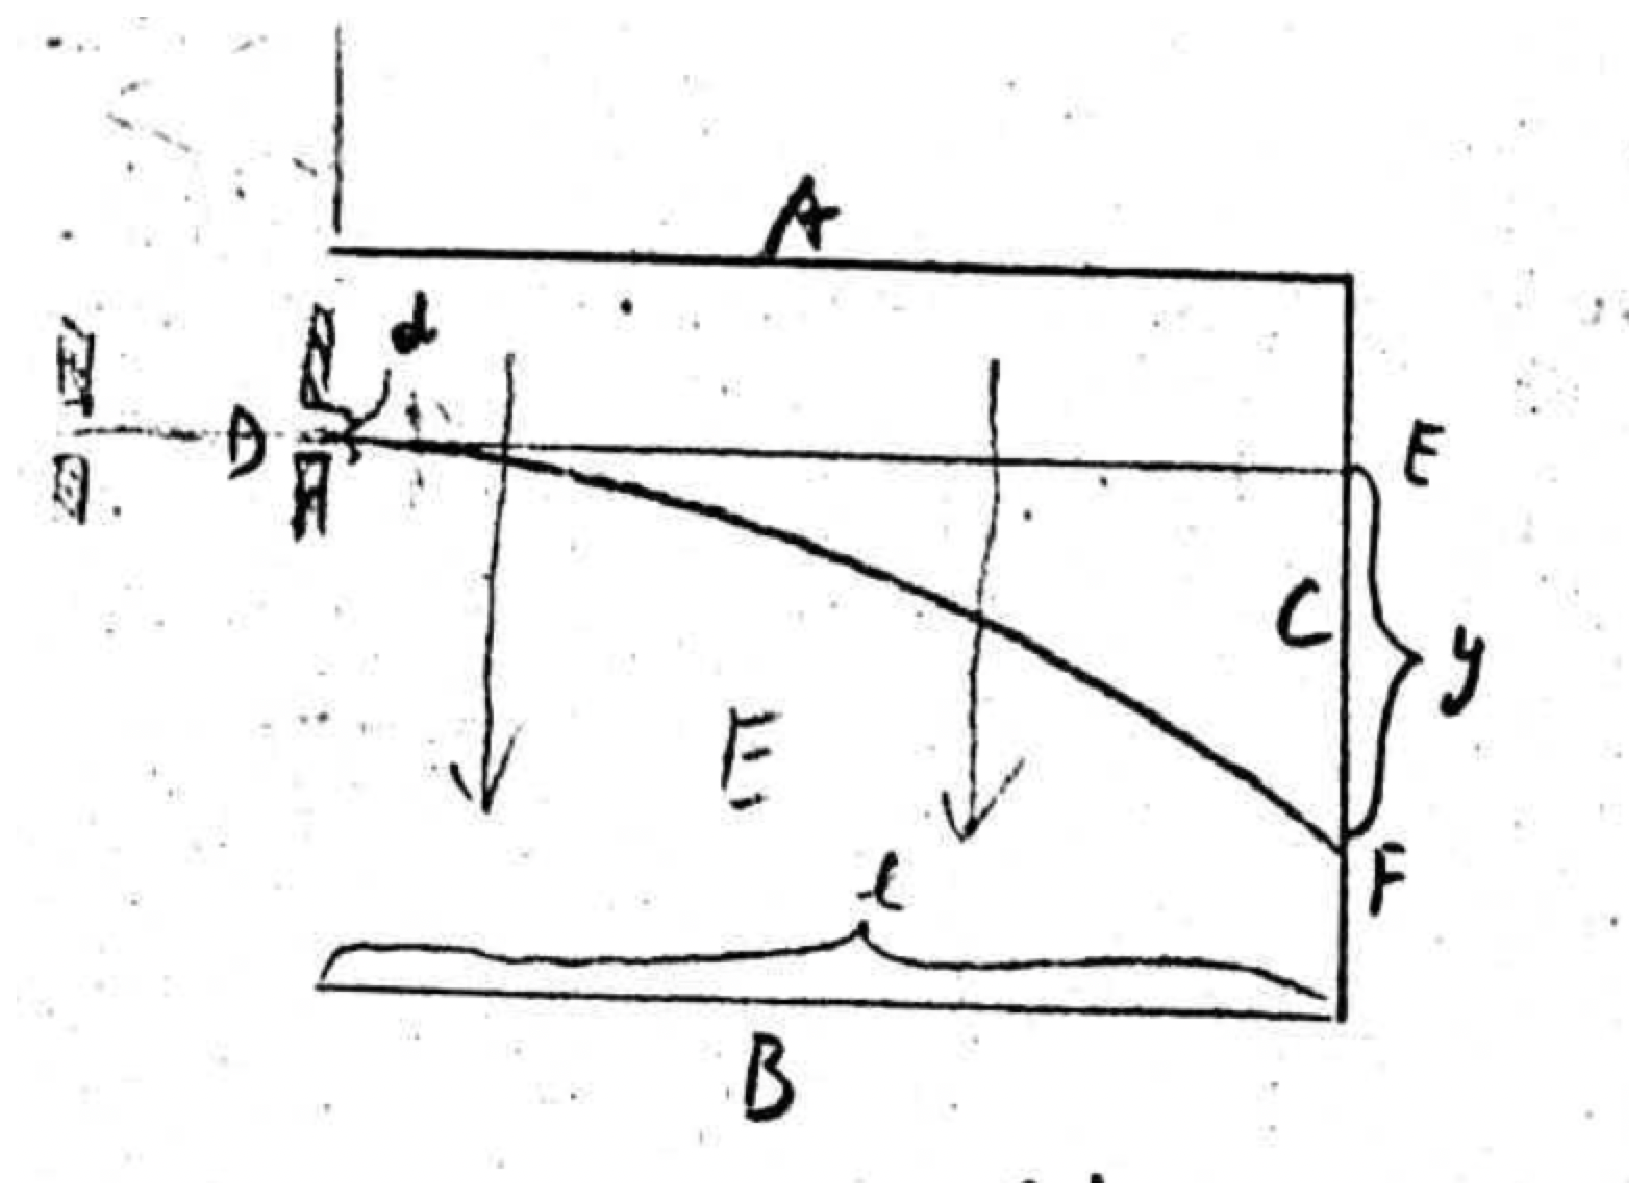
\includegraphics[scale=0.2, trim = 0mm 0mm 0mm 0mm, clip]{1934WeizsaeckerElectrical}
 \caption{From the letter by \letterKPA{von Weizsäcker}{Popper}{6}{12}{1934}[360-21] \label{fig:weizsaeckerelectrical}}
\end{figure}

%Otherwise an electron arriving higher on the screen might simply have entered the field at a different position rather than having had a different momentum.


To infer the momentum from the impact point, the electron's path through the field must be fixed with sufficient precision. This requires diaphragms at $D$ (\cref{fig:weizsaeckerelectrical}). But narrowing the diaphragm increases diffraction. If the slit has width $d$, then the transverse spread $\Delta y$ at the detector is constrained both by the slit width and by the transverse momentum uncertainty generated by diffraction:
%
\begin{equation*}
\Delta y > d,
\end{equation*}
\begin{equation*}
\Delta y = \frac{\Delta p_y}{mv}l,
\end{equation*}
with
\begin{equation*}
d\Delta p_y \geq h.
\end{equation*}
It follows that
\begin{equation*}
(\Delta y)^2 \geq \frac{h}{mv}l.
\end{equation*}
%
Thus the diaphragms required to define the beam path blur the screen point that is supposed to determine the momentum \letterKPAp{Von Weizsäcker}{Popper}{6}{12}{1934}[360-21].


This transverse uncertainty also affects the longitudinal motion. Since $y$ depends on the flight time $t=l/v$, an uncertainty in $y$ implies an uncertainty in $v$:
\begin{equation*}
\frac{\Delta y}{y} = 2\frac{\Delta v}{v}.
\end{equation*}
%
This yields an uncertainty in the longitudinal momentum, $\Delta p_x=m\Delta v$, and in the reconstructed coordinate $x=vt$. Combining these uncertainties, \vW\ concluded that the product $\Delta p_x\Delta x$ cannot be reduced below the order of Planck's constant. For small deflections, his calculation gives
%
\begin{equation*}
\Delta p_x \Delta x > \frac{l^2}{y^2}h,
\end{equation*}
%
so that no violation of the uncertainty relation is obtained. Larger deflections require an additional angular correction, but do not alter the conclusion \letterKPAp{Von Weizsäcker}{Popper}{6}{12}{1934}[360-21]. The same arrangement that makes the impact point interpretable as a momentum measurement also prevents the earlier position from being sharply reconstructed. \VW\ therefore concluded that Popper had not supplied a realizable experiment capable of undercutting the uncertainty principle.\letterKPAp{Von Weizsäcker}{Popper}{6}{12}{1934}[360-21].


%The decisive point was structural, not merely practical. 

% \VW\ stressed that this was the reverse of Heisenberg's example of an initial position determination followed by a momentum measurement in a field. \citep[21--22]{Heisenberg1930} In both temporal directions, the uncertainty relation blocks the combination of sharp momentum knowledge and retrodictive position knowledge required by Popper's argument. 

%\subsection{Heisenberg's Countereply}
%
%In his reply of \datedm{10}{12}{1934}, Heisenberg enclosed \vW's criticism and opened by assuring Popper that, after discussing the matter with \vW, he had had the note corrected so that it no longer appeared unjustifiably sharp.\letterKPAp{Heisenberg}{Popper}{10}{12}{1934}[305-32] Heisenberg summarized \vW's result as follows: the proposed \s{Aussonderung} of electrons by an electric field is not a genuine momentum measurement in Popper's sense, since the experiment cannot yield an exact trajectory of the particle before the momentum measurement. He then turned to Popper's analogous suggestion of using a light filter instead of an electron spectrometer. As he put it, the optical case could be treated in the same way. The filter would select light of a given frequency, but it would not prepare quanta with an infinitely sharp momentum.
%
%Heisenberg suggested that Popper consider reflective resonance filters, such as sodium or mercury vapor, following Wood's \origg{Reststrahlenverfahren}. Such a device reflects or re-emits radiation near the resonance frequency, while other components of the incident light are not selected in the same way. Thus a broad beam can be reduced, for example, to the sodium D-lines. Yet the selected light is never strictly monochromatic. Since the filtering process depends on the excitation and subsequent de-excitation of the reflecting atom, the resonance line has a finite width. Heisenberg expresses this by writing that the inaccuracy of the momentum of the light quantum is given by
%\begin{equation*}
%\Delta p = \frac{h\Delta\nu}{c^2}.
%\end{equation*}
%The precise form of the factor is less important for his argument than the point that a finite frequency width $\Delta\nu$ entails a finite momentum width $\Delta p$.
%
%Heisenberg then connects this linewidth to a temporal indeterminacy. The probable residence time of the light quantum in the reflecting atom is determined by the lifetime of the corresponding excited state:
%\begin{equation*}
%\Delta t = \frac{1}{\Delta\nu}.
%\end{equation*}
%Thus, even if the later position of the light quantum were known with precision, its position before reflection could not be reconstructed exactly, because the moment at which it was in the reflecting atom remains indeterminate by $\Delta t$. This temporal indeterminacy produces an uncertainty in the reconstructed position before reflection, and Heisenberg concludes that
%\begin{equation*}
%\Delta x \Delta p \sim h.
%\end{equation*}
%In the optical case, therefore, the uncertainty relation is preserved for the same structural reason as in \vW's analysis of the electrostatic analyzer: the physical procedure that selects momentum also prevents an exact retrodiction of the earlier position.
%
%Heisenberg finally made explicit that Popper's \s{nichtprognostischen Messungen} had not, in his view, been shown to be impossible in general merely by \vW's discussion. Rather, what had been shown was that the particular examples Popper had proposed did not work. He nevertheless thought it plausible that the impossibility of such measurements was a very general feature of quantum mechanics. He remarked that a proof of this point would presumably amount to the content of an important paper in mathematical physics, and added that he feared Popper had here followed one of those misleading errors by which he himself, Bohr, and others had been tempted since 1927, before they came to believe that they had really understood quantum theory. He closed by thanking Popper for sending his book, which he had not yet been able to study carefully.\letterKPAp{Heisenberg}{Popper}{10}{12}{1934}[305-32]


% As he put it, the optical case could be treated in the same way. The filter would select light of a given frequency, but it would not prepare quanta with an infinitely sharp momentum, the time of the passage wouild be lost is the time of pasage, since the filter ....  In his reply of \datedm{16}{12}{1934}, 



\section{The Hermann-\vW Correspondence on Popper's Thought Experiment}
%
In his reply of \datedm{10}{12}{1934}, Heisenberg enclosed \vW's letter and then dismantled Popper's attempt to invert his \TE by replacing the electron beam with a light beam and using a light filter to select light quanta that already possessed the \s{right} momentum \letterKPAp{Heisenberg}{Popper}{10}{12}{1934}[305-32]. In response, Popper sent Heisenberg a revised version of the second communication summarizing the debate \citep{Popper1934c}. He conceded that \vW's argument against the electrostatic selector was correct but defended his idea of using a light-quantum filter against Heisenberg's objections \letterKPAp{Popper}{Heisenberg}{16}{12}{1934}[305-32]. Heisenberg did not reply further. But Popper persisted. He suggested another experimental arrangement, whose examination Heisenberg delegated to his other assistant Hans Euler. Popper envisaged two diffraction gratings inclined in opposite directions, each imposing a separate selection condition, hoping to select both wavelength and direction of the incoming light quanta. Euler replied on \datef{4}{2}{1935} by showing that the two gratings form a single coherent interference system and cannot be treated separately\footnote{Popper--Euler Correspondence, Karl Popper Archives 293-29}.

\subsection{Hermann's Letter to \vW}
%
While the Leipzig group had begun to tire of Popper's stubbornness, \vW received a review copy of \LdF from the \emph{Physikalische Zeitschrift}. Given their dispute during the preceding months, however, he declined to review the book and instead sent it to Hermann. Writing to \vW from Østrupgaard in Denmark, Hermann asked for clarification regarding his response to Popper's \TE \letterGHp{Hermann}{\W}{5}{3}{1935}[14]. In particular, she requested an offprint of his reply to Popper in \emph{Die Naturwissenschaften}, since she wanted to determine how far Popper had addressed his objections. Hermann noticed that Popper’s thought experiment in the main text of \LdF appeared essentially unchanged from the version he had explained to her in Prague, probably at the 1934 philosophy congress, and from the version discussed in \emph{Die Naturwissenschaften}. The two appendices, however, seemed to her to reflect Popper’s discussion with Weizsäcker \letterGHp{Hermann}{\W}{5}{3}{1935}[14]. 

This was not, in fact, the case, since Appendices \rom{6} and \rom{7} had already been written before \vW's response. Nevertheless, as we have seen, Popper does seem to have anticipated a possible objection to his momentum-measuring apparatus and had already proposed a momentum filter as a replacement. Hermann, however, pointed out that this would not solve the problem:

\qt{Both \textins{appendices} concern the possibility of detecting a corpuscle in such a way that the position and time of impact, for example on a strip of film or by means of a point counter, are determined precisely, together with the direction and magnitude of the momentum with which the particle arrives. In the first case, the aim is to determine the magnitude of the momentum for a given direction; in the second, to determine the direction as well. What is more, the measurements are supposed to be such that they do not apply merely to the interval \myemph{between} the momentum measurement and the position measurement, during which, incidentally, no further disturbance may occur; rather, they are also supposed to determine the exact trajectory of the corpuscle for the time \myemph{before} the momentum measurement, so that, on the basis of some earlier collision, the trajectory of another particle can then be predicted with an accuracy exceeding the uncertainty relations. The decisive trick by which this physically inadmissible prediction is to be forced is, in the first appendix \textins{VI}, a momentum selection, that is, a selection of the particles in which this momentum is found, to be carried out on a nonmonochromatic, parallel-directed beam of particles, and specifically in such a way that the momenta of the selected particles, or their momentum component in the direction of the beam, are not changed}{Es geht in beiden um die Möglichkeit, ein Korpuskel derart aufzufangen, dass dabei der Ort und der Zeitpunkt des Auftreffens etwa auf dem Filmstreifen oder mit einem Spitzenzähler1 und zugleich Richtung und Betrag des Impulses, mit dem das Teilchen auftrifft, genau bestimmt wird, im ersten darum, bei gegebener Richtung den Impulsbetrag, im zweiten darum, auch die Richtung festzulegen. Und zwar sollen die Messungen so sein, dass sie nicht etwa nur für den Zeitraum zwischen Impuls- und Ortsmessung gelten, in dem im übrigen keine weitere Störung stattfinden darf, sondern sie sollen auch für die Zeit vor der Impulsmessung die genaue Bahn der Korpuskel bestimmen, sodass dann auf Grund irgend eines früheren Zusammenstosses die Bahn eines anderen Teilchens mit einer die Unbestimmtheitsrelationen übersteigenden Genauigkeit vorhergesagt werden kann. Der entscheidende Trick, mit dem diese physikalisch unzulässige Voraussage erzwungen werden soll, ist im ersten Anhang eine Impul- saussonderung (d. h. Auslese der Teilchen, an denen dieser Impuls angetroffen wird), die an einem nichtmonochromatischen, parallel gerichteten Teilchenstrahl vorgenommen werden soll, und zwar so, dass dabei die Impulse der ausgesonderten Teilchen (bzw. ihre Impulskomponente in der Strahlrichtung) nicht verändert wird}[\letterGHp{Hermann}{\W}{5}{3}{1935}[14\me]]
%
Hermann clearly identified the central flaw of Popper's arrangements: Popper needs to determine not only the electron's momentum \emph{between} the momentum and position measurements, but also its momentum \emph{before} the first momentum measurement, in order to reconstruct the collision time at $S$ and thereby predict the entire trajectory of the correlated particle $B$ testable at $Y$.

Hermann jotted down some still undeveloped ideas to ask for \vW's opinion. They are articulated in three points.

\begin{enumerate}
\item Hermann first points out that, according to \qm, Popper cannot use the momentum measurement at $X$ to retrodict the earlier trajectory of the $A$-particle with arbitrary precision. At this point, she tentatively locates Popper's mistake in the assumption that a momentum component can be measured without an uncontrollable disturbance of that very component: \qt{An exact momentum measurement will therefore be able to determine either the momentum before the measurement or the momentum after it, but not both}{Eine genaue Impulsmessung wird also nur entweder den Impuls vor, oder den nach der Messung festlegen können, nicht aber beides} \letterGHp{Hermann}{Weizsäcker}{5}{3}{1935}[14]. Otherwise, she argues, an exact momentum measurement would determine both the momentum before and the momentum after the measurement, thereby immediately violating the uncertainty relations. Yet Hermann does not rest content with this apparatus-specific disturbance argument. She asks whether the impossibility of such a measurement can be derived more generally from the deeper requirement of wave-particle duality. Popper appeals to various devices--a film strip or tip counter for registering the particle, a filter for a light beam, and spectral analysis in an electric field for an electron beam--but Hermann is unsure how, in each case, the failure of the proposed apparatus follows from the necessary interplay of wave and particle descriptions.

\item For Hermann the deeper source of Popper's mistake was indeed his misunderstanding of wave-particle duality. From the \LdF, one can gather that Popper treats the $\psi$-function as a wave-like statistical description of ensembles of particles: \qt{The error in this consideration is this: according to Heisenberg's derivation, the uncertainty relations follow from the dualism experiments and from the compulsion issuing from them to apply features of the wave picture to every atomic process, and features of the corpuscular picture to every wave propagation}{Der Fehler dieser Überlegung: Die Unbestimmtheitsrelationen folgen gemäss Heisenbergs Ableitung aus den Dualismus-Experimenten und der von ihnen ausgehenden Nötigung, auf jeden atomaren Vorgang auch Merkmale des Wellenbildes, auf jede Wellenausbreitung auch Merkmale des Korpuskelbildes anzuwenden} \letterGHp{Hermann}{Weizsäcker}{5}{3}{1935}[14]. The \UR therefore limit not merely the composition of ensembles, but the applicability of classical state descriptions to individual systems. The probability interpretation of the wave function captures only one aspect of \qm: it specifies what can be said when one passes from one measurement context to another. After the momentum measurement, the system is in an eigenstate of the momentum operator; in this case the corresponding value is not merely probable but fixed. But if one asks what would be obtained by measuring position, for instance what position would be found after a momentum context has been fixed, the wave function supplies only a probability distribution over possible outcomes: \qt{Popper fails to recognize this side of Bohr's complementarity}{Diese Seite der Bohrschen Komplementarität verkennt Popper} \letterGHp{Hermann}{Weizsäcker}{5}{3}{1935}[14].

%Relative to a fixed observation context, by contrast, the wave function provides an exact state description, independent of probability statements. 

\item Given these premises, Hermann turns to the problem of past trajectory reconstructions. Popper is not merely unable to reconstruct the trajectory of the $A$-particle before the momentum measurement at $X$; it also makes no sense, in the relevant physical sense, to speak of a particle's trajectory \emph{between} the momentum and the position measurement. In general, retrospective trajectory calculations ignore wave-particle duality by restricting themselves to the intuitive features of only one picture, usually the corpuscular picture, and then joining together quantities fixed in distinct measurements. Popper's electron--photon interaction cannot be described solely as a corpuscular collision. The interaction between the light quantum and the electron is described within the corpuscular picture in accordance to energy and momentum conservation, but the propagation of the scattered light must be described within the wave picture. An apparatus like Heisenberg-\vW's $\gamma$-ray microscope is therefore needed to determine how the wave-optical propagation is correlated with the corpuscular scattering event. Optical instruments of this kind fix either the point of origin or the direction of propagation of the scattered light, but not both with arbitrary precision. Hermann therefore concludes that Heisenberg’s \qt{much-debated remark}{viel umstrittene Äusserung}, according to which the past trajectory was a matter of taste, was unfortunate \letterGHp{Hermann}{Weizsäcker}{5}{3}{1935}[14].
\end{enumerate}
%
As we shall see, \vW would express some reservations about point (1). Otherwise, however, the letter contained the outline of Hermann's critique of Popper's interpretation of \qm, which she would articulate in both her long article on \qm \citep{Hermann1935} and her review of \LdF \citep{Hermann1935a}.

\subsection{\VW's Reply to Hermann}

\begin{wrapfigure}{r}{0.20\textwidth}
\centering
\includegraphics[scale=0.3, trim=0mm 0mm 0mm 0mm, clip]{spitz}
%\citetrackerfalse
\caption{\VW's scheme for a tip counter; from \cite[485]{Herrmann2019}\label{fig:spitz}}
\end{wrapfigure}

Hermann’s tone is markedly different from Popper’s self-assured manner. Despite having a much more sophisticated knowledge of \qm, she proceeds cautiously, asking at nearly every step whether \vW would agree with her remarks. \VW thus plays the expert to whom Hermann turns for technical clarification \letterGHp{Weizsäcker}{Hermann}{13}{3}{1935}[15]. For instance, at Hermann's request, \vW explains what a tip counter is, an instrument with which Hermann was apparently unfamiliar\label{tipcounter}. In such a counter, the sensitive electrode is a fine metal tip $S$ \origg{Spitze}, maintained at a high potential difference relative to the surrounding conductive wall $W$ of the gas-filled counter chamber (\cref{fig:spitz}). An ionizing particle passing sufficiently close to the tip produces primary ions in the gas; the strong electric field near the tip then amplifies this ionization into a discharge. The discharge registers that a particle has passed through the small sensitive region around the tip and thus gives a relatively sharp practical determination of the place and time of its passage. As \vW adds, \qt{A photographic plate, pinhole aperture, or the like therefore performs exactly the same function as the tip counter}{Eine photographische Platte, Lochblende o. ä. tut also genau dieselben Dienste wie er} \letterGHp{Weizsäcker}{Hermann}{13}{3}{1935}[15].

\begin{wrapfigure}{l}{0.35\textwidth}
\centering
\includegraphics[scale=0.3, trim=0mm 0mm 0mm 0mm, clip]{vWfilter}
%\citetrackerfalse
\caption{\VW's scheme for a spectral analyzer; from \cite[483]{Herrmann2019}\label{fig:electric}}
\end{wrapfigure}

The system, or any straightforward modification of it, is not suitable for measuring momentum, contrary to Popper's claim. For this reason, in his paper \vW had proposed a measurement by the Doppler effect. He agrees with the result of Hermann's critique in point (1) of her letter, but slightly revises her diagnosis of the failure \letterGHp{Weizsäcker}{Hermann}{13}{3}{1935}[15]. On Hermann's diagnosis, an exact momentum measurement cannot determine both the incoming and the outgoing momentum, because the measurement must involve an uncontrollable \emph{disturbance} of the measured momentum component itself \letterGHp{Weizsäcker}{Hermann}{13}{3}{1935}[15]. According to \vW, however,  we know the initial state of the electron and the incident light-quantum, it is possible to determine the incoming and outgoing momenta. The issue is that an exact momentum measurement takes a \emph{finite time}, so that the instant of the measuring collision is not known. Consequently, a later position cannot be traced back through the measuring process to an earlier position with arbitrary precision. Even granting Popper exact knowledge of the momentum before and after the measuring interaction, he still cannot reconstruct the collision time at $S$, because he does not know how long the particle moved with the pre-collision momentum and how long with the post-collision momentum \letterGHp{Weizsäcker}{Hermann}{13}{3}{1935}[15].

Popper's selection of electron momenta in an electric field does not improve the situation. \VW reiterates a simplified version of the argument that he and Heisenberg had developed in correspondence with Popper (\cref{fig:electric}). He adds that Popper's filter has the same structure as the field-deflection measurement discussed by Heisenberg for a magnetic field in his textbook \citep[21]{Heisenberg1930}. In Heisenberg's example, a beam of charged particles passes through a slit of width $d$, traverses a homogeneous magnetic field over a distance $a$, and is deflected by an angle $\alpha$, from which the longitudinal velocity, and hence the momentum, can be inferred:

\begin{equation*}
\alpha=\frac{aHe}{mcv}.
\end{equation*}
%
\VW schematizes the same problem by considering a beam entering a field region through an aperture of width $d$ and arriving at a point $P$ after a displacement $y$. The arrival point can function as momentum information only because the field maps different momenta onto different deflections. But this inference presupposes that an aperture has defined the incoming beam: its finite width limits the geometrical accuracy of the reconstruction, while too narrow an aperture produces diffraction. Heisenberg therefore obtains, for the magnetic-field case, the constraints

\begin{equation*}
\Delta \alpha \gtrsim \frac{d}{l+a} \quad \quad \Delta \alpha \gtrsim \frac{\lambda}{d},
\end{equation*}
%
which jointly prevent an arbitrarily sharp determination of both the beam localization and the direction of propagation. The same limitation applies to \vW's simplified diagram: the later arrival at $P$ and the displacement $y$ do not allow one to reconstruct a precise earlier position independently of the conditions that made momentum selection possible. In both cases, the field-deflection measurement yields momentum information only at the cost imposed by aperture width and diffraction, so that the uncertainty relation is restored.

Popper had proposed light-filter arrangements as well, but \vW notes that he initially had no clear account of what sort of filter should be used for light. \VW explains to Hermann Heisenberg's argument against the use of resonance fluorescence to filter the photon momentum in some detail \letterGHp{\vW}{Hermann}{13}{3}{1935}[15]. He recounts that, Popper devised further experimental arrangements, probably referring to the arrangement refuted by Euler. For a time, it had become, as \vW put sarcastically it, \q{a parlor game \origins{Gesellschaftsspiel} for us in Leipzig, to refute Popper's setups} \letterGHp{\vW}{Hermann}{13}{3}{1935}[15]. The basic idea behind these refutations, he suggests, is this: the corpuscular picture is applicable only as long as one can also replace \s{corpuscle} by \s{wave packet}. Any arrangement capable of undercutting the uncertainty relation would have to make possible a wave packet with

\begin{equation*}
\frac{\Delta \pos}{\Delta \lambda}<1.
\end{equation*}
%
This is fundamentally absurd in classical wave kinematics, which requires $\Delta \pos$ to be larger than $\Delta \lambda$: The narrower the spatial extension of a wave packet ($\Delta \pos \to 0$), the wider the spread of different constituent wavelengths (forcing $\Delta \lambda \to \infty$). Yet \vW remains cautious about whether this \q{recipe for refuting Mr. Popper} can be transformed into a compelling general argument. In the end, he suggests, one must appeal to the quantum-mechanical formalism as a whole, which Popper seems not to have understood \letterGHp{Weizsäcker}{Hermann}{13}{3}{1935}[15].

With respect to point $2$, \vW tends to agree with Hermann, although his lack of familiarity with Popper's book prevents him from making the claim with complete confidence: \qt{With Popper, it has already happened to me once that, with the best will in the world, I could not quite work out \emph{what} he had actually misunderstood}{Es ist mir bei Popper ja schon einmal so gegangen, dass ich beim besten Willen nicht genau herausbrachte, \emph{was} er eigentlich missverstanden hatte} \letterGHp{Weizsäcker}{Hermann}{13}{3}{1935}[15]. At that time, Popper had assumed that his \s{non-prognostic measurements} were \qt{a generally known and accepted matter}{eine allgemein bekannte und anerkannte Sache} \letterGHp{Weizsäcker}{Hermann}{13}{3}{1935}[15]. Hermann's question was whether Popper's mistake lay in treating the wave function statistically, as if wave--particle duality applied only to ensembles rather than to individual quantum processes. Here, however, \vW cannot satisfy Hermann's request to provide an experiment in which wave-particle duality is manifested in a single system. In processes involving individual particles, wave--particle dualism can hardly be demonstrated except by repeating the experiment. The reason may be that all measurements ultimately culminate in the determination of a position at a time, that is, a spacetime coincidence, thereby allowing a corpuscular description of the individual case.

%His reply to point $3$ is strikingly brief: he simply states that he fully agrees. The point that would become central to Hermann’s public refutation of Popper is therefore already present in her letter, while \vW merely endorses it without further elaboration.  He cannot think of a single experiment that would count as proof of the wave picture. 

\section{Hermann on Popper in \emph{Die naturphilosophischen Grundlagen der Quantenmechanik}}


On \datedm{19}{3}{1935}, Heisenberg wrote his last letter to Popper, explaining that all the considerations developed in his previous letter applied to transmitted light as well \letterKPAp{Heisenberg}{Popper}{19}{3}{1935}[305--32]. With this, Heisenberg declared the matter closed. Yet one might say that that a more systematic \s{public} answer of the Leipzig group to Popper came not from Heisenberg or \vW, but from Hermann. In his reply to Hermann, \vW does not comment on point (3) of her letter, although this point would become the core of her published refutation: quantum mechanics allows the reconstruction of measurement processes, but that such reconstructions must not be confused with the reconstruction of past trajectories. 

As previously mentioned, Hermann ultimately traced the failure of Popper's set-up to his misunderstanding of wave-particle duality \NGQd{\S2}. Popper applies the wave description to the probability distribution of an ensemble of particles, and the particle description to individual particles. By contrast, according to Hermann, each individual electron and photon must be described under the dual aspect of corpuscle and wave: \qt{In this relative character of the quantum mechanical mode of description lies the new and amazing natural-philosophical aspect that is here introduced into the view of nature. What it consists of can best be understood on the basis of a thought experiment treated by a pupil of Heisenberg}{In diesem relativen Charakter der quantenmechanischen Beschreibungsweise liegt das naturphilosophisch Neue und Verblüffende, das hier in die Naturbetrachtung eingeführt worden ist. //110// Worin er besteht, läßt sich am besten an Hand eines Gedankenexperiments auffassen, das ein Schüler HEISENBERGs durchgerechnet hat} \NGQ{110--11}{257}. 

The student in question is of course \vW. A few years earlier, von \citet{Weizsacker1931} published a paper on the localization of an electron by means of a microscope, developing a modified version of \citets{Heisenberg1927} famous microscope argument. In Heisenberg's original version, the measurement of position leaves the electron's momentum indeterminate because of the uncontrollable momentum transfer involved in the scattering process. \VW's treatment, by contrast, emphasizes a different point: measurements of position and momentum require two incompatible experimental arrangements. \VW's aim was primarily to substantiate Heisenberg's analysis through detailed calculations; Hermann, by contrast, used a qualitative version of the \TE to express the central conceptual novelty of \qm \citep{Filk2016}. 

\subsection{The \HW Microscope}
%
Since Hermann's presentation seems to presuppose some working knowledge of the apparatus, I will provide a more didactic account. Hermann considers an electron moving along the object plane $L$, identified with the $x$-axis (\cref{fig:HW}). The relevant conjugate quantities are therefore its position \pos along this plane and the corresponding momentum component \mom. To measure the electron, one illuminates it with a light quantum prepared in a plane-wave state, that is, with a photon of well-defined momentum. The situation can be simplified by assuming that only a single photon in each run is involved. The central point is that the light quantum involved in the electron's illumination must be described under the dual aspect of wave and particle. As a particle, it collides elastically with the electron according to the classical laws of impact, where momentum conservation applies: both the light quantum and the electron are deflected, and their changes of momentum are equal in magnitude and opposite, in particular in the $x$-direction. As a wave, it is deflected by the electron, enters the microscope, is propagated through the lens according to the classical laws of optics, and reaches a scintillating screen $S$. 

\begin{figure}
\centering
\includegraphics[scale=0.3, trim=0mm 0mm 0mm 0mm, clip]{WHdiagram}
\caption{A schematic of the \WH microscope\label{fig:HW}. Left (original from \cite[115]{Weizsacker1931}): $S$ in the image plane. Right (reconstructed): $S$ in the focal plane}  
\end{figure}
%
It is useful to spell out a few details of classical optics that remain implicit in Hermann's account. A lens takes parallel rays and bends them toward a single point. Let us assume that the lens has fixed optical properties, determined by its refractive index $n$ and by the radii of curvature $R_1$ and $R_2$ of its surfaces. These properties determine the focal length $f$, the distance from the lens to the focal point at which rays entering parallel to the optical axis are brought together. For a thin lens in air, this relation is given by the lens maker's equation:

\begin{equation*}
\frac{1}{f}=(n-1)\left(\frac{1}{R_1}-\frac{1}{R_2}\right).
\end{equation*}
%
The \emph{focal length} $f$ is therefore a constant determined by the lens and the surrounding medium. It should be distinguished from the \emph{image distance}, that is, the distance from the lens's principal plane to the plane at which rays diverging from a given object point are brought together at the corresponding image point. The image distance depends not only on the lens but also on the position of the object plane $L$. If $d_o$ denotes the distance from $L$ to the lens, and $d_i$ the distance from the lens to the plane in which the corresponding image is formed, the thin-lens equation gives

\begin{equation*}
\frac{1}{f}=\frac{1}{d_o}+\frac{1}{d_i}.
\end{equation*}
%
Thus, once the lens and the object plane $L$ are fixed, $d_o$ is constant, and the corresponding image distance $d_i$ is thereby determined (\cref{fig:HW}). The same lens can nevertheless be used in two distinct arrangements, depending on the position of the screen $S$ relative to the lens: \begin{inparaenum}[(a)] \item if the lens-to-screen distance is $d_i$, then $S$ lies in the \emph{image plane} \item if the lens-to-screen distance is $f$, than $S$ lies in the \emph{focal plane} \end{inparaenum}. 


%All light entering the lens passes through both the focal and image planes, but different families of rays converge in each plane at $P'$\ref{fig:HW}. In the arrangement on the left, rays arriving at the lens from the same direction, originating from different points $P_1, P_2, P_3 \ldots$, are focused at a single point $P'$ on the screen $S$, which is positioned at the focal distance $f$. In the arrangement on the right, each point $P$ in the object plane $L$ is mapped onto a corresponding point $P'$ in the image plane $S$, located further away at the image distance $d_i$. The lens brings parallel rays to a focus at the focal distance. Rays emanating from a finite-distance object at $P$ arrive at the lens already diverging; the lens must first compensate for this divergence so that the rays converge only at a greater distance, at the image distance $d_i$, after which they diverge again. 


The same lens may be used in two arrangements. With the screen at the focal distance $f$, rays entering the lens with the same direction are focused to the same point $P'$ on the screen. With the screen at the image distance $d_i$, rays originating from the same object point are focused to the corresponding image point $P'$. Since rays arrive at the lens already diverging, the lens must first compensate for this divergence so that the rays converge only at a greater distance. This classical optical duality constrains the operation of the \HW microscope \citep[\S10]{Hermann1935}. The apparatus functions as a preparation device for incoming photons, selecting them either by position or by direction:
%
\begin{itemize}
\item $S-\text{lens}=d_i$: In the image-plane arrangement, the optical system groups together photons scattered from the same position $P$, even though they leave $P$ in different directions within the aperture. These directions are recombined at the image point $P'$. From the mark on the plate at $P'$, one can infer the position $P$ of the electron at the time of its collision with the photon. This description presupposes that a spherical wave spreads out from the point of collision and that the whole aperture of the microscope contributes to the image. In the corresponding corpuscular description, however, this means that no definite direction can be assigned to the photon after scattering. The momentum transferred to the electron therefore cannot be exactly determined. Immediately after the collision, the electron must be described approximatively by a spherical wave function $\psi$ that assigns it a relatively sharp position but a less sharply determined momentum.\todo{check}

\begin{itemize}
\item To obtain a very precise position measurement $\Delta \pos$, one needs a large lens aperture $2\epsilon$, so that the microscope collects more of the spherical wave coming from $P$ and thereby localizes its origin more precisely.\footnote{If the aperture angle $2\epsilon$ is small, the lens receives only a narrow cone of the spherical wave. Then many nearby points would produce nearly indistinguishable wavefronts at the lens, and the resulting image point is diffraction-broadened. The origin of the spherical wave is therefore only poorly localized} A large $\epsilon$, however, means that the scattered photon may have entered the microscope from within a wide range of directions. This produces a large, unavoidable uncertainty in the momentum transferred to the electron, so that $\Delta \mom$ is correspondingly large. In this arrangement, therefore, only the probability of finding the particle with a given direction of motion can be specified.
\end{itemize}

\begin{equation*}
\Delta \pos \sim \frac{\lambda}{\sin\epsilon}, \quad \Delta \mom \sim \frac{h}{\lambda}\sin\epsilon.
\end{equation*}

\item $S-\text{lens}=f$: In the focal-plane arrangement, the optical system groups together photons with the same outgoing direction, even though they may have been scattered from different points $P_1,P_2,P_3,\ldots$ in the object plane $L$. These photons are focused onto the same point $P'$ of the focal plane $S$. In this arrangement, the point $P'$ therefore determines the direction in which the scattered light entered the microscope. The scattered photon travels mostly upward, so its momentum has a large $y$-component and, if it is slightly inclined, a smaller $x$-component. If $\alpha$ is the angle between the scattered photon's direction before it reaches the lens and the vertical optical $y$-axis, then the transverse momentum component of the photon is $p_{P,x}=p_P\sin\alpha$. If the photon's transverse momentum before the collision is known, conservation of momentum fixes the corresponding change in the electron's momentum $p_{E,x}$. The electron wave function $\psi$ is therefore represented, in this momentum context, approximately as a plane wave with relatively sharp momentum but indeterminate position.

\begin{itemize}
\item To obtain precise momentum information, the apparatus must distinguish closely spaced incident directions. The lens maps the physical scattering angle $\alpha$ in the object space to the refracted angle $\vartheta$ in the image space. Since the focal-plane mark resolves only a narrow angular spread $\delta\vartheta$ of the refracted light, the smaller $\delta\vartheta$, the more precisely the photon's original direction, and thus its transverse momentum, can be determined. This gain, however, leaves the point of origin in the object plane $L$, and thus the position of the scattering event, indeterminate: only the probability of finding the particle at a given point can be specified.
\end{itemize}

%However, the resolving power of the focal-plane mark is limited to a narrow angular spread $\delta\vartheta$ of the refracted light. This instrumental limit determines the irreducible uncertainty $\delta\alpha$ of the initial scattering angle. 

\begin{equation*}
\Delta \mom \sim \frac{h}{\lambda}\delta\vartheta, \quad \Delta \pos \sim \frac{\lambda}{\delta\vartheta}.
\end{equation*}
\end{itemize}
%
It is worth noting that Hermann’s analysis presupposes two aspects of wave-particle duality, thus two levels of \s{complementarity}. Moving beyond Hermann’s own terminology, the first may be called \begin{inparaenum}[(a)]
\item \emph{inter-contextual}: the incompatibility between image-plane and focal-plane arrangements familiar from classical wave optics acquires direct significance for the attribution of state to particles: image or focal plane arrangements are \emph{complementary} in the strict sense, they register either the point of origin or the direction of propagation of waves, and hence either position or momentum of particles \NGQ{128}{284}. The second is \item \emph{intra-contextual}, internal to each context: once an arrangement has been chosen (image or focal plane), the interplay between the wave and corpuscular descriptions yields the corresponding \emph{uncertainty} trade-off between the position and momentum of particles \NGQ{129}{284}. \end{inparaenum}

If no photographic plate $S$ is introduced, the photon is not registered, and a third description is required, which might be called \emph{pre-contextual}, that is, prior to the choice of the observational context \NGQ{135}{258}. Hermann explains this in a short note set in smaller type, worth examining in some detail. Before the collision, the photon and electron may still be described by a total wave function that is the product of their respective wave functions, $\phi$ and $\psi$. In Hermann's notation:\footnote{I rely on \letterGH{Hermann}{Scholz/Kratzer}{8}{7}{1936}[28]}

\begin{equation*}
\varphi\cdot\psi=\sum_k a_k \varphi_k \sum_i b_i \psi_i
\end{equation*}
%
After the collision, however, the wave function of the composite system is, in general, no longer given by the product of two independently assigned wave functions one for each subsystem, but by a \q{linear combination}, that is, a superposition or weighted sum of such products \NGQ{113}{258}:

\begin{equation*}
\sum_{ik} c_{ik}\,\varphi_i\psi_k
\end{equation*}
%
where the coefficients no longer factorize into separate coefficients for the two subsystems, $c_{ik} \neq a_k b_i$. In Hermann's idealized thought experiment, the fixed initial momenta together with momentum conservation, and the geometry of the optical apparatus, establish one-to-one correlations between the electron and the photon. Accordingly, the coefficients may be written with a single index,

\begin{equation*}
\sum_n c_n\,\varphi_n\psi_n ,
\end{equation*}
%
where corresponding electron and photon wave functions are paired by the same index. The coefficients determine the probabilities of the correlated joint outcomes: $|c_n|^2$ is the probability that a measurement yields the correlated pair $\varphi_n\psi_n$, that is: if the photon is found in the state $\psi_n$, then the electron is in the corresponding correlated state $\varphi_n$. In particular, the same joint wave function may be expanded in terms of either the correlated momentum eigenfunctions or the correlated position eigenfunctions, depending on whether one chooses to measure momentum or position:

\begin{equation*}
\sum_n c_n^{(p)}\,
\varphi_n^{(p)}
\psi_n^{(p)}
=
\sum_n c_n^{(x)}\,
\varphi_n^{(x)}
\psi_n^{(x)}.
\end{equation*}
%
One may distinguish two equivalent representations of the same joint state. If the registration plane is placed at the \emph{focal plane}, the joint state is naturally represented by an expansion of the correlated momentum eigenfunctions. Each term then correlates a photon momentum eigenstate $\psi_n^{(p)}$ with the corresponding electron momentum eigenstate $\varphi_n^{(p)}$, reflecting momentum conservation,

\begin{equation*}
p_E+p_P=P_{\mathrm{tot}}.
\end{equation*}
%
If, instead, the registration plane is placed at the \emph{image plane}, the same joint state is more naturally represented by an expansion of the correlated position eigenfunctions. Each term then correlates a photon position eigenstate $\varphi_n^{(x)}$ with the corresponding electron position eigenstate $\psi_n^{(x)}$, reflecting the geometrical relation established by the optical arrangement between the collision point and the registration on the screen,

\begin{equation*}
x_E-x_P=\text{constant}.
\end{equation*}
%
The important point is that these are not two independent descriptions of independently characterized systems, but two representations of one and the same joint state. Depending on whether one adopts the momentum or the position representation, the state is expanded in terms of momentum- or position-correlated eigenstates, respectively, using the corresponding orthogonal system.

One can already glimpse the correlation structure that, as we shall see, would become central to discussions of quantum mechanics only a few months later \citep[sec.~5.2]{Filk2016}. After the collision, the resulting state is generally no longer a simple product of an electron state and a photon state, but a linear combination in which each term correlates a particular state of the electron with a corresponding state of the scattered photon: \qt{These various possibilities, among which observation decides, are merged on an equal footing by a symbolic addition \origins{Summation} into a combined wave function that develops in a phase space \origins{Phasenraum} determined by the degrees of freedom of both systems}{In einer symbolischen Summation werden diese verschiedenen Möglichkeiten, unter denen die Beöbachtung entscheidet, als gleichberechtigt zu einer Wellen-die Beobachtung entscheidet, als gleichberechtigt zu einer Wellen·funktion zusammengeschlossen} \NGQ{137}{270}. In Hermann’s example, if one \emph{chooses} to measure the photon’s position, one can predict with certainty the electron’s position; if one instead \emph{chooses} to measure its momentum, one can predict with equal certainty the electron’s momentum. However, these two alternative descriptions, since they belong to different and incompatible observational contexts, are necessarily counterfactual and cannot be \emph{combined} into a real position-cum-momentum state of the electron.
 
Hermann's goal is to show that a registration event, a mark $P'$ on the photographic plate $S$, has no determinate physical meaning by itself. Its significance depends on the \emph{reconstruction} of the entire optical arrangement (the lens, the focal point, the position of the planes, etc.) that correlates it either with a direction of propagation or with a point of origin. In particular, if the plate $S$ is placed in the focal plane, at distance $f$ from the lens, the lens maps parallel rays, and hence a definite propagation direction, onto a point on the plate. The mark $P'$ is then interpretable as momentum information. Its precision depends on the angular spread $\delta\vartheta$ of the rays contributing to that mark. If, by contrast, the plate $S$ is placed in the image plane corresponding to the object plane, at distance $d_i$ determined by the thin-lens equation, the lens maps object points onto image points. The same kind of mark $P'$ is then interpretable as position information, since it indicates the point $P$ from which the photon was scattered. Its precision depends on the resolving power of the image, and thus on the aperture angle $2\epsilon$. 

%: the smaller $\delta\vartheta$, the more sharply the corresponding momentum component is determined.



\subsection{Hermann Against Popper: Measurement Reconstruction vs.\ Trajectory 
Reconstruction}
%
At this point, Hermann is able to articulate her position regarding the principle of causality following the advent of \qm. The principle of causality can no longer be understood to require sharp \emph{predictions} of future measurement outcomes, since quantum mechanics generally yields only statistical predictions. Nevertheless, it must be presupposed as the condition for unambiguous \emph{retrodiction} from an already registered measurement outcome $P'$ to the microscopic quantity, say \pos or \mom \NGQ{105-106}{272}. As in classical physics, this retrodiction requires a \emph{causal reconstruction}: only through a theory of the measuring apparatus can one draw an unambiguous inference from a measuring result, such as a pointer reading, to a property of the object measured \citep[\S12]{Hermann1935}. However, \qm makes this dependence more radical. Because of wave-particle duality, in quantum mechanics one may reconstruct the measurement as yielding either \pos or \mom, but not both within a single observational context. The choice of context is therefore \emph{free}, in accordance with wave-particle duality; once that context has been chosen, however, the reconstruction is \emph{necessary}, as required by the \apr principle of causality \citep[sec.~22.3.1]{Crull2022}. It is this interplay that Hermann, in the closing section of her paper, famously called a \s{splitting of truth} \origg{Spaltung der Wahrheit} \NGQd{\S18}.

After the choice has been made, each causal reconstructions, say, from the mark $P'$ on  $S$ back to the photon’s position, is indirectly testable through the statistical predictions they yield for the electron. A few pages later---probably after her correspondence with \vW about Popper---Hermann added a small-print note warning against confusing two types of causal reconstruction---legitimate \s{measurement reconstructions} and illegitimate \s{trajectory reconstructions}:
%
\qt{The retrospective inferences \origins{Rückschlüsse} underlying these indirect predictions, however, must not be confused with those familiar inferences \origins{Rückschlüssen} that apparently allow one to determine a physical system for a past time segment with accuracy exceeding the uncertainty relations. Thus it appears as though one could, for instance, escape the limits on measurement accuracy by taking two position measurements on an electron in quick succession, or by first determining its momentum and shortly thereafter its position, in order then to calculate from the results of both measurements together the exact trajectory of the electron for the time interval between the two measurements, and thus determine with arbitrary accuracy its respective position and momentum for this time}{Die Rückschlüsse, die diesen mittelbaren Voraussagen zu Grunde liegen, dürfen allerdings nicht mit jenen bekannten Rückschlüssen verwechselt werden, die für einen vergangenen Zeitabschnitt ein physikalisches System anscheinend mit einer die Unbestimmtheitsrelationen übersteigenden Genauigkeit zu bestimmen gestatten[\cite[15]{Heisenberg1930}]. So scheint es, als könne man sich den Schranken der Meßgenauigkeit etwa dadurch entziehen, daß man an einem Elektron kurz nacheinander zwei Ortsmessungen vornimmt, oder daß man zunächst seinen Impuls und kurz darauf seinen Ort bestimmt, um dann aus den Ergebnissen beider Messungen zusammen die genaue Bahn des Elektrons für die Zeitspanne zwischen beiden Messungen zu berechnen, seinen jeweiligen Ort und Impuls für diese Zeit also mit beliebiger Genauigkeit zu bestimmen}[\NGQ{121}{262}]
%
Hermann argues that the after-the-fact reconstruction of a particle trajectory differs fundamentally from the retrospective reconstruction of the measurement process. According to Hermann, \emph{trajectory reconstructions} ignore the dualism of wave and particle descriptions; in particular, they ignore what I have labeled the inter-contextual aspect of this dualism:

\qt{This posterior \origins{nachträgliche} construction of an electron trajectory differs from the inferences \origins{Rückschlüsse} that are necessary for the interpretation of a measurement in that it takes no account of the duality of the wave and particle picture, limits itself to the intuitive features of one of these pictures and, since each single observation makes reference to both pictures and hence admits unlimited use of neither, fixes these features through two different observations. In this way one apparently succeeds in combining the variables belonging to different observational contexts into a single description of the physical system. In contrast to this, the causal inference that determines the state of the observed from that of the measuring instrument must take duality into account in the interpretation of a measurement. For it is essential for the process of measurement that every atomic process also exhibits a wave character, and every wave motion also a corpuscular character. The single observation of the measuring instrument that grounds the inference to the object of measurement determines in which way the wave and particle picture delimit each other in the present interpretation}{Diese nachträgliche Konstruktion einer Elektronenhahn unter· scheidet sidl von den Rückschlüssen, die zur Interpretation einer Messung erforderlich sind, dadurch, daß sie dem Dualismus von Wellen· und Partikelbild keine Rechnung trägt, sich auf die an· schauliehen Merkmale eines dieser Bilder beschränkt und, da jede einzelne Beobachtung auf heide Bilder Bezug nimmt und daher keines von ihnen unbeschränkt anzuwenden gestattet, diese Merk· male durm zwei verschiedene Beobachtungen festlegt. Auf diesem Weg gelingt es anscheinend, die zu verschiedenen Beobachtungs. zusammenhängen gehörenden Bestimmungsstücke in einer einzigenBeschreibung des physikalischen Systems zu vereinigen. Im Gegensaß dazu muß bei der Interpretation einer Messung der Kausalsmluß, der aus dem Zustand des Meßinstruments den des beobamteten Objekts entnimmt, den Dualismus berücksichtigen. Denn für den Vorgang der Messung ist es wesentlich, daß jeder atomare Vorgang auch Wellen<harakter, jede Wellenbewegung auch korpuskularen Charakter zeigt. Die eine Beobachtung des Meß· apparats, die dem Rücksmluß auf das Meßobjekt zu Grunde liegt, bestimmt dabei, in welcher Weise Weilen· und Partikelbild ein· ander bei der vorliegenden Interpretation begrenzen}[\NGQ{121--22}{262}]
%
%For Hermann, wave–particle duality has two distinct consequences. At the inter-contextual level, it determines which measurement can be performed: one must choose an experimental arrangement in which the object is described either under the conditions appropriate to a position measurement or under those appropriate to a momentum measurement. The two contexts cannot be fused into a single, context-independent description of the system.
%
%%Hermann contrasts this illegitimate reconstruction with the interpretation of a measurement, the \qt{retrospective inferences}{Rückschlüssen} required for the interpretation of a measurement. 
%
The \emph{trajectory reconstruction}, by combining features fixed through two different observational contexts, momentum \emph{and} position, tries to unite determinations that in fact belong to different observational contexts within a single description of the physical system. The \emph{measurement reconstructions}, from the mark of an indicator to the value of a quantity of the observed object, momentum \emph{or} position, must account for wave–particle dualism. This, Hermann continues, was precisely the lesson of the microscope example:

\qt{The significance of this contrast follows from the relative character of the quantum-mechanical mode of description. Since every physical description and explanation of processes is valid only relative to its respective observational context, the calculation of, say, a corpuscular trajectory that combines the variables of different observational contexts into a single representation remains physically vacuous precisely to the extent that it exceeds the uncertainty relations: it is uncheckable and provides no basis for future predictions.\textins{$^{\ast}$} The controversial representation Heisenberg gave of this situation—that it is purely a matter of taste \origg{Geschmacksfrage} whether one should assign physical reality to such trajectory calculations—is therefore to be amended in the sense that such calculations disregard the quantum-mechanically crucial relation that each specification of a physical variable \origins{physikalische Bestimmung} bears to the respective observational context and, in this sense, become physically meaningless. Conversely, the possibility of checking, even indirectly, the causal claims that arise in the interpretation of a measurement process depends on the fact that this interpretation does justice to duality, and thus implicitly to the relative character of quantum mechanics}{Die Bedeutung dieses Gegensates ergibt sich aus dem nur relativen Charakter der quantenmechanischen Beschreibungsweise. Da jede physikalische Beschreibung und Erklärung von Vorgängen nur relativ zum jeweiligen Beobachtungszusammenhang gilt, so bleibt die Berechnung etwa einer Korpuskelbahn, die die Be-stimmungen verschiedener Beobachtungszusammenhänge zu einer Darstellung zusammenfaßt, eben in dem Maß, wie sie über die Unbestimmtheitsrelationen hinausgeht, physikalisch leer: Sie ist unkontrollierbar und gibt keine Anhaltspunkte für Vorausberechnungen. ${ }^{10}$ Die umstrittene Darstellung, die Heisenberg diesem Sachverhalt gegeben hat, es sei eine reine Geschmacksfrage, ob man einer solchen Bahnberechnung physikalische Realität zuordnen solle, ist demnach dahin zu berichtigen, daß diese Rechnung die quantenmechanisch entscheidende Beziehung jeder physikalischen Bestimmung auf den jeweiligen Beobachtungszusammenhang außer Acht läßt und insofern physikalisch bedeutungslos wird. Umgekehrt hängt die Möglichkeit einer, wenn auch nur mittelbaren Kontrolle der Kausalbehauptungen, die bei der Interpretation eines Messungsvorgangs auftreten, daran, daß diese Interpretation dem Dualismus und damit implizite dem relativen Charakter der Quantenmechanik gerecht wird}[\NGQ{122}{263}\tm]
%
%Like \citep{Schlick1931}.%However, Hermann's contextualist reading is more subtle than Schlick's blunt operationalist approach. For Schlick, a past trajectory cannot be tested; for Hermann, the two context-dependent determinations cannot be combined
%
The reference marked by the asterisk $^{\ast}$ is again to p.~15 of \citets{Heisenberg1930} Chicago lectures. As we have seen, for Heisenberg, the question whether physical reality can be assigned to such a reconstructed trajectory is merely a \s{matter of taste}. For Hermann, by contrast, it was, so to speak, a \s{matter of context}. According to Hermann, at the \emph{inter-contextual} level, the trajectory calculation ignores the quantum-mechanically decisive fact that every physical determination is relative to a specific observational context. Put in slightly modern terms, one may construct either a $x(t)$-history or a $p(t)$-history, but not a hybrid history (\ie, a trajectory) that treats both as simultaneously valid descriptions of the same individual process. At the \emph{intra-contextual} level, once one of these histories has been selected, the alternative history can be reconstructed only probabilistically. If the chosen context fixes a position history, then the corresponding momentum history is not available as a determinate trajectory, but only as a distribution of possible momentum values. Conversely, if the chosen context fixes a momentum history, then the corresponding position history remains indeterminate and can be specified only probabilistically. 

The premises for Hermann's critique of Popper are now established. She adds a footnote to the passage just quoted, marked here by an asterisk $^{\ast}$, applying this analysis to Popper's 1934 paper in \NW. As we have seen, Popper's strategy was based on a very permissive interpretation of Heisenberg's matter-of-taste remark: \qt{One has attempted, however, to use such calculations of trajectories to derive predictions in a similarly indirect manner as happens in the interpretation and checking of measurements, and thereby to overcome the limits of the uncertainty relations}{Es ist allerdings der Versuch gemacht worden, solche Bahnberechnungen zu benutzen, um in ähnlich mittelbarer Weise, wie es bei der Interpretation und Kontrolle von Messungen geschieht, Voraussagen abzuleiten und in ihnen die Schranken der Unbestimmtheitsrelationen zu überwinden} \NGQ{123\fn{10}}{263\fn{10}}. As Hermann suggests, Popper's setup is structurally similar to Hermann's own. In both cases, after the electron--photon collision, the two particles are described by the same kind of pre-contextual joint state. Popper then \emph{chooses} a context, that is, to measure first the momentum of the electron and later its position in order to reconstruct the trajectory and use conservation laws to predict the photon trajectory. Extending Hermann's analysis, one can argue that since Popper fails to recognize that a choice of context has been made, his attempt ultimately fails on two levels:

\begin{itemize}
\item At the \emph{intra-contextual level}, after the electron--photon collision, a momentum measurement on the photon selects the momentum representation of the joint state. By momentum conservation, this also fixes the corresponding momentum of the electron. But precisely within this momentum context, the electron's position is indeterminate. Popper therefore cannot reconstruct the electron's position-cum-momentum trajectory \emph{before} the first momentum measurement at $X$.

\item At the deeper \emph{inter-contextual level}, Popper tries to combine this momentum determination with a later position measurement, as if the two results belonged to a single classical history of the same particle. However, in \qm state attributions at each instant are irreducibly tied to in general mutually exclusive experimental contexts; thus it is physically meaningless to stitch them together to form a context-independent trajectory. Thus, even the notion of a trajectory \emph{between} the momentum measurement and the position measurement at $X$ has no well-defined quantum-mechanical meaning.
\end{itemize}
% 
As already anticipated in her letter to \vW, Hermann claims that the roots of Popper's mistake can be understood only if one reads not only Popper's 1934 paper but also his 1935 book: \qt{the real basis of this mistake, as only the more detailed discussions in Popper's book \textit{Logik der Forschung} (Vienna, 1935) show, lies in a misapprehension of the dualism experiments and their consequences}{ie den physikalischen Fehler des POPPERschen. Der eigentliche Grund dieses Fehlers liegt, wie erst die ausführlicheren Darlegungen in POPPERs Buch „Logik der Forschung“ (Wien 1935) zeigen, in einer Verkennung der Dualismus-Experimente und ihrer Konsequenzen} \NGQ{263\fn{10}}{123\fn{10}}. In the book, Popper interprets the wave description as referring to an ensemble \origg{Schar} and the particle description as referring to an individual member of that ensemble\footnote{Indeed, \citet{Popper1936a} will later attempt to demystify  \s{complementarity} in this way}. For Hermann, by contrast wave and particle are complementary descriptions of the same individual system under different experimental conditions: 

%$(\psi, \phi) \rightsquigarrow P(\phi \mid \psi)$.

%($\psi \rightsquigarrow P(p, q)$)

%gives  

%The statistical character of quantum mechanics therefore does not reside in the fact that the wave function only refers to an ensemble of systems but in the probabilistic relation between complementary experimental contexts. 


%In Popper's interpretation, the wave-description refers to the probability distribution over an ensemble, while the particle description is an individual member of that ensemble.   For Hermann the wave and particle descriptions concern the same individual system limiting the the contextual natura Consequently, the wave function does not describe a probability distribution over particles. It assigns the probabilities of the outcomes that would be obtained in an incompatible experimental arrangement. 


%For Popper the wave function $\varphi$ a wave-like probability distribution over an ensemble \origg{Schar} of \emph{particles} with unknown position and momenta \citep[\S5]{Hermann1935}. For this reason acoording. Hermann objects that this misconstrues the significance of wave-particle duality applies to every single system. 

%For this reason Popper: The statistical interpretation therefore applies not within a single context but only to the transition between incompatible contexts. A state prepared in the momentum context determines only the probabilities of the outcomes in a position context, and conversely:


%Acoording Hermann objects that this misconstrues the significance of wave-particle duality. Wave and particle are not alternative descriptions of different members of an ensemble, but complementary descriptions of the same individual system in different experimental contexts. 

%Popper interprets the wave function as a probability distribution over an ensemble of particles existing within a single experimental arrangement.

%statistical interpretation of \qm rests on the idea that the function $\varphi$ describes a wave-like probability distribution over an ensemble \origg{Schar} of \emph{particles} \citep[\S5]{Hermann1935}. According to Hermann, however, this interpretation misconstrues the significance of wave-particle duality. The wave and particle descriptions apply to the same individual physical system, although which description is appropriate depends on the experimental context:

\qt{Popper is led by the probabilistic interpretation of wave functions to apply these quantum-mechanical state descriptions and the uncertainty relations given with them, strictly speaking, only to ensembles of physical systems, while assuming that a suitably selected individual system is not bound by the uncertainty relations. In doing so, he fails to recognize that, on the basis of the dualism experiments, the applicability of classical concepts is already restricted for each individual elementary process in accordance with the uncertainty relations, and that, accordingly, wave functions are perfectly usable for describing the states of individual systems. That this use of wave functions is compatible with their probabilistic interpretation rests once again solely on the relative character of the quantum-mechanical mode of description: on the one hand, the wave function is completely determined by the values of those physical quantities that have a sharp value for the system in the present observational context. To this extent, it characterizes the system quantum-mechanically relative to the present observational context. On the other hand, the probabilistic interpretation of wave functions leads to those determinations that remain from the classical-intuitive description in accordance with the correspondence principle and that determine which statements can be made for the transition from one observational context to another}{POPPER läßt sich durch die Wahrscheinlichkeitsdeutung der Wellenfunktionen dazu verleiten, diese quantenmechanischen Zustandsbeschreibungen und die mit ihnen gegebenen Unbestimmtheitsrelationen streng genommen nur auf Scharen physikalischer Systeme anzuwenden, für ein einzelnes geeignet herausgegriffenes System aber keine Bindung an die Unbestimmtheitsrelationen anzunehmen. Er verkennt dabei, daß auf Grund der Dualismus-Experimente schon für jeden einzelnen Elementarvorgang die Anwendbarkeit der klassischen Vorstellungen den Unbestimmtheitsrelationen entsprechend beschränkt ist und daß entsprechend die Wellenfunktionen durchaus zur Zustandsbeschreibung einzelner Systeme brauchbar sind. Daß diese Verwendung der Wellenfunktionen mit ihrer Wahrscheinlichkeitsinterpretation vereinbar ist, beruht wieder allein auf dem relativen Charakter der quantenmechanischen Beschreibungsweise: Die Wellenfunktion ist einerseits vollständig bestimmt durch die Werte derjenigen physikalischen Größen, die beim augenblicklichen Beobachtungszusammenhang für das System einen scharfen Wert haben. Insofern charakterisiert sie das System quantenmechanisch relativ zum gegenwärtigen Beobachtungszusammenhang. Andererseits führt die Wahrscheinlichkeitsdeutung der Wellenfunktionen zu denjenigen Bestimmungen, die von der klassisch-anschaulichen Beschreibung gemäß dem Korrespondenzprinzip bestehen bleiben und die festlegen, welche Aussagen für den Übergang von einem Beobachtungszusammenhang in einen anderen gemacht werden Kenny}[\NGQ{123--24\fn{10}}{263--64\fn{10}}]
%
The same point is reiterated in Hermann’s review of Popper’s book in \jt{Physikalische Zeitschrift}, which appeared in July. The statistical interpretation therefore does not consist in assigning a wave-like probability distribution to an underlying ensemble of particles. Rather, the wave function $\phi$ has a dual role. At the \emph{intra-contextual} level, within each \OC provides a contextual description of the individual system, determined by those quantities that are sharply defined in that observational context. Its probabilistic interpretation, by contrast, is \emph{inter-contextual}: $\phi$ determines the probability distribution for the observables that would become sharp only in another, incompatible \OC{}s. Popper’s probabilistic interpretation is misleading because it remains \emph{non-contextual}: it treats the wave function $\phi$ as a statistical description of an ensemble of \emph{trajectories} of particles that may still be conceived as possessing definite, context-independent joint position-and-momentum histories.


%the momentum (position) operator 

%The statistical interpretation therefore does not consist in assigning a wave-like probability distribution to an underlying ensemble of particles. Rather, it becomes applicable only when one considers the probabilistic relations governing the transition from one observational context to another. 




%probability is binary (relational)—it links two contexts, the preparation context \psi and the measurement context \phi. 


%\citep{Hermann1935b}

\section{Conclusion: Hermann and Popper after EPR}
%
%Hermann’s long study appeared in the \emph{Abhandlungen der Fries’schen Schule} and was also distributed as a separately printed booklet or offprint. 

Hermann’s paper was completed in March 1935, the same month in which the EPR paper was submitted to the \emph{Physical Review} \citep{Einstein1935}. At roughly the same time, Popper came into contact with Einstein through a mutual acquaintance\footnote{\letterae{Busch}{Einstein}{28}{4}{1935}[34-338]; \letterKPA{Einstein}{Popper}{15}{6}{1935}[292-12]; \letterae{Popper}{Einstein}{18}{7}{1935}[19-126]}. During the spring of 1935, Popper worked on a response to the criticisms from the Leipzig group, expanding it into a longer manuscript, again titled \art{Zur Kritik der Ungenauigkeitsrelationen}. It cannot be ruled out that the July publication of \citets{Hermann1935a} review of the \Lo in the \jt{Physikalische Zeitschrift} reinforced his conviction that a public stance was necessary. Weisskopf’s account of Einstein’s recent paper criticizing quantum mechanics led Popper to hope that Einstein would prove more receptive than Heisenberg. Popper therefore decided to send Einstein the manuscript \letteraep{Popper}{Einstein}{29}{8}{1935}[19--127]. However, Popper's hope was ultimately disappointed: Einstein rejected the proposed experimental setup on the same grounds as Heisenberg and \vW \letteraep{Einstein}{Popper}{11}{9}{1935}[19-130]. However, he also unwittingly provided Popper with an alternative.

Lacking an extra offprint of the paper to enclose, Einstein explained the EPR setup to Popper. This scenario is somewhat similar to Popper's thought experiment. Two systems, $A$ and $B$, interact for a short time and are then separated. After the interaction, they are described by the joint non-factorizable wave function $\psi_{AB}$. A measurement is performed on $A$, and quantum mechanics assigns different $\psi_B$-functions to $B$ depending on which measurement is performed on $A$. By freely choosing to measure either the position or the momentum of $A$, one can predict either the corresponding position or the corresponding momentum of the distant system $B$ with certainty. \q{if, upon freely choosing to do so [that is, without interfering with it], I am able to predict something, then this something must exist in reality} \letteraep{Einstein}{Popper}{11}{9}{1935}[19-130]\footnote{Translation from \cite[459]{Popper1959}}. Einstein's argument comes close to what Popper was searching for: although Einstein cannot predict the future trajectory of $B$, he appears to suggest that \q{the system $B$ has indeed a definite momentum and a definite position co-ordinate} \letteraep{Einstein}{Popper}{11}{9}{1935}[19-130].

\citets{Bohr1935} reply to Einstein was published a few weeks later, in October. Hermann learned about EPR indirectly from Bohr's paper, but she quickly noted the similarities with her own $\gamma$-microscope setup. \qt{Einstein's objection}{Einsteinsche Einwand}, she wrote in correspondence, is likewise based on the \s{linearly combined} wave function of a composite system, \qt{if I have understood him correctly based on Bohr's answer}{wenn ich ihn nach Bohrs Antwort richtig verstanden habe} \letterGHp{Hermann}{Scholz/Kratzer}{8}{7}{1936}[28]. Hermann therefore had a ready reply. Since the experimental arrangements for measuring position and momentum are mutually exclusive, the predictions concerning the second system are necessarily counterfactual: \qt{The feature determined by measurement characterizes the system only in the new observational context, not in the old one}{Das durch Messung festgestellte Merkmal charakterisiert das System nur im neuen Beobachtungszusammenhang, nicht im alten. Dieser alte Beobachtungszusammenhang war also nicht unvollstän-dig[, und es liegt nicht so, dass durch die Messung nur etwas aufgedeckt worden wäre, was uns im alten Beobachtungszusammenhang entgangen wäre} \letterGHp{Hermann}{Scholz/Kratzer}{8}{7}{1936}[28]. \Qm does not license the \q{combination \origins{Vereinigung}} of determinations belonging to different alternative possible observational contexts into a single state description: \qt{every state description is only relative to the respective observational context}{jede Zustandsbeschreibung nur relativ zum jeweiligen Beobachtungszusammenhang} \letterGHp{Hermann}{Scholz/Kratzer}{8}{7}{1936}[28].

Popper and Hermann may have had another opportunity to meet at the Second International Congress for the Unity of Science, held in Copenhagen in June 1936, where \citet{Hermann1936} delivered a short address. However, there is no evidence that the encounter left any trace. They both left continental Europe shortly thereafter, in 1937. They revisited \qm only after the war at the turn of the 1950s \citep{Henry-Hermann1948,Popper1951}. However, whereas Hermann seems to have moved on, absorbed in political and pedagogical commitments, for Popper this marked the beginning of a full-scale return to the philosophy of \qm after the debacle of the 1930s \citep{DelSanto2019}. Popper began writing the material on \qm in 1951--56, shortly before the publication of the first English edition of the \Lo in 1959. Part of this material was included in the appendices, while the rest became a separate \textit{Postscript} to the \Lo, which reached galley proofs in 1956--57 but remained unpublished. 

In the new English edition of the \Lo, the main text of the chapter on \qm was left untouched; however, Popper sought to make amends for his previous mistakes with new footnotes and appendices marked with starred numbers. Popper acknowledged what \vW had pointed out to him: trajectory reconstruction was not possible \q{\myemph{before} the first of these measurements}, that is, the momentum measurement \citep[242\fnstar{3}\me]{Popper1959}. Without this, Popper's \TE fails. However, Popper continued to hold that \q{non-predictive measurements determine the path of a particle only \myemph{between} two measurements,} such as a measurement of momentum followed by one of position \citep[242\fnstar{3}\me]{Popper1959}. Popper seems not to have appreciated, and quite possibly not to have read, Hermann's deeper critique that quantum mechanics does not license trajectory reconstructions in general.  This is not simply an oversight. Popper’s interpretation of \qm has significantly changed after the war. The frequency interpretation of probability has been replaced by the propensity interpretation \citep{Popper1957,Popper1959}, the issue of determinism by that of realism. However, Popper never ceased to believe that Heisenberg’s concession that the existence of past trajectories was a \s{matter of taste} opened a crack in the \s{orthodox interpretation} that Popper hoped to widen.


%the propensiy, the issue of determinis by that of realis, Stull Popper appears never to have abandoned the conviction that the very notion of past trajectories was not merely a \s{matter of taste}, nor was it meaningless, as Schlick maintained. They are an essential component of \qm. For Popper, Heisenberg's concession was the crack that  \s{Copenhagen interpretation} measuring agencies with the physical object under investigation

The 1956--57 draft of the \emph{Postscript}, and even more clearly a 1966 text \citep{Popper1967}, later incorporated in expanded form into the printed volume \citep{Popper1982}, conceded that in \qm \emph{predictions} of future trajectories are statistical, with dispersions related by the Heisenberg formulae. However, testing these predictions requires measurements, and \q{\emph{these measurements are retrodictions}} (\cite[25]{Popper1967}; \cite[60]{Popper1982}); such retrodictions are, in Popper's view, reconstructions of particle trajectories. Since \qm is a theory about the probabilities of trajectories, trajectories must be real, \ie, particles thus \s{possess} sharp positions and momenta at every instant. While the \UR forbid combining incompatible arrangements to \emph{prepare} an ensemble of particles with the same position and momentum without producing a scatter, Popper insisted that it must be possible to combine the corresponding arrangements to \emph{measure} the very scatter predicted by the \UR \citep[21]{Popper1967}.  According to \citet[III-17]{Popper1982}, this is precisely what the EPR \TE demonstrates: If upon freely choosing to measured either position or momentum on the system $A$, I can determine with certainty either position or momentum of $B$ without disturbing it, then $B$ possesses definite position and momentum, even though the theory does not enable us to predict them at the same time.

\todo{??}
In Popper's view \citets[697]{Bohr1935} objection surreptitiously changes the  argument by introducing the idea of a \s{non-mechanical disturbance} \citep[445]{Popper1959}. If we choose to measure the momentum of $A$, we can determine the momentum of $B$ with arbitrary precision without disturbing it; however, in doing so we forgo the possibility of measuring its position. Had we instead chosen to measure position, the opposite would have been the case: \q{The arrangements are exclusive of each other (or \s{complementary}), the argument continues, and so we cannot combine the two spaces \textelp{} into one} \citep[149]{Popper1982}. According to Popper, however, EPR had already conceded this premise: position and momentum cannot both be measured in a single run. The real issue is that, according to Bohr, the counterfactual status of the unperformed measurement prevents us from inferring simultaneous elements of reality. Popper, however, regarded this prohibition as contrary to common sense \citep[150]{Popper1982}: if I can freely choose to determine either your weight or your height with certainty without disturbing you, then it is unreasonable to deny that you possess both simultaneously \citep[150]{Popper1982}. Popper's choice of counterexample is somewhat careless: height and weight can be measured within the same experimental arrangement in a single run, whereas in \qm, position and momentum cannot. Nevertheless, it vividly captures what was his deeper concern.

%\todo{??}

%In retrospect, the debate over whether belief in the reality of past trajectories was a \s{matter of taste} was one of the earliest philosophical controversies generated by quantum mechanics. 

As Popper put it, testing a statistical theory requires \s{\emph{retrodictions}}. He equated retrodictions with reconstructions of particle \s{\emph{trajectories}}: trajectories must be real, and particles must therefore possess simultaneous position and momentum \emph{despite} the mutual exclusivity of the corresponding experimental arrangements. Hermann identified the questionable premise on which this argument rests. Retrodictions are indeed indispensable for testing \qm, but they reconstruct \s{\emph{measurement}} processes: \emph{because} the corresponding experimental arrangements are mutually exclusive, particles cannot possess simultaneous position and momentum, and trajectories are therefore meaningless. Although the controversy over trajectories later largely receded\footnote{See, however, the criticism of Popper in \cite{Feyerabend1968,Feyerabend1969} and his defense in \cite[366--67]{Ballentine1970}}, it foreshadowed the deeper philosophical issue that emerged after EPR. Popper shared Einstein's fear that, unless the physical state could be fully detached from the experimenter's intervention, one would have to accept the \q{intrusion of subjectivism into physics} \citep[2, 5]{Popper1982}. Hermann, by contrast, like Bohr, recognized early on that quantum mechanics requires a weaker form of detachment. State attribution depends on the experimenter's free choice among mutually exclusive experimental arrangements, yet this does not render the physical state \s{subjective}. Once the experimental arrangement is fixed, the state attribution is objectively determined \s{relative to that observational context} \citep[380--81]{Henry-Hermann1948}.


%\todo{Feyerabend}
% \hide{that, in a one-slit experiment, a definite trajectory can be reconstructed retrospectively from the position preparation and the subsequent momentum measurement. In modern preparation--measurement language, Hermann would object that the position preparation determines a diffracted wave, not a particle with an unknown momentum component. The subsequent measurement licenses the attribution of a definite particle momentum to the outcome, but not the retrospective attribution of a trajectory}


%After the slit the system is a spherical wave, in a position preparation context there is no determinate momentum. After the The context only allows to interpret the spot on the screen as a momentum measurement, rather than a position measurement

%the preparation merely reveals a pre-existing trajectory.
%the preparation defines the context within which a causal reconstruction is meaningful. If Hermann’s “context” is interpreted as what we now call a preparation procedure, then the contextuality lies at the source, not primarily at the detector. The preparation fixes the state (or ensemble); the subsequent measurement merely samples one of the complementary observables. That seems closer to Hermann’s actual discussion than the modern tendency to associate contextuality exclusively with the measurement apparatus.

%With a fixed slit, the screen coordinate can be interpreted as a momentum measurement because the initial position is well defined. With a movable slit, the initial position is no longer well defined, so the same screen coordinate loses its unambiguous momentum interpretation and is naturally regarded simply as a position detection.

%Consider a single slit experiment:  


%    relative to the actual preparation and measurement performed


%The single slit prepares the particle in a position context. The screen then performs a momentum measurement. From the initial position preparation and the final momentum outcome one may reconstruct the particle’s intermediate trajectory. However, this reconstruction is valid only within that particular experimental context. Had the final measurement instead been one of position, a different reconstruction would have been obtained. Thus what is reconstructed is not a context-independent history of the particle but the history associated with the actual preparation-and-measurement sequence.
\bibliographystyle{sn-basic}
\bibliography{natbib}

%\citetrackerfalse
%
%\printshorthands
%\printbibliography

\end{document}
